\subsection{离散时间马氏链}

马尔可夫性 $\leftrightarrow$ 已知现在,过去与未来不相干/独立

\begin{definition}[(离散时间)马氏链]\label{def:M_1}
    称 $S$ 值随机过程 $\{X_n,n\geq 0\}$ 为马氏链,若 $X$ 满足以下马氏性:$\forall n\geq 0,x_0,x_1,\cdots,x_n,y\in S$,
    \[
    \PP(\underbrace{X_{n+1}=y}_{\text{未来}}|\underbrace{X_0=x_0,\cdots,X_{n-1}=x_{n-1}}_{\text{过去}},\underbrace{X_n=x_n}_{\text{现在}})=\PP(X_{n+1}=y|X_n=x_n)\label{eq:M1}\tag{$M_1$}
    \]
    其中 $X_0$ 的分布称为 $X$ 的初始分布
\end{definition}

\begin{definition}
    当 $S$ 为有限集,称链为有限链,当 $S$ 为无限集,称链为无限链
\end{definition}

注:改写 $(M_1)$
\[
LHS=\PP_{X_n=x_n}(X_{n+1}=y|X_0=x_0,\cdots,X_{n-1}=x_{n-1})
\]
\[
RHS=\PP_{X_n=x_n}(X_{n+1}=y)
\]
\[
\begin{aligned}
    M_1 &\Leftrightarrow \{X_{n+1}=y\}\ind_{\{X_n=x_n\}}\{X_0=x_0,\cdots,X_{n-1}=x_{n-1}\}\\
    &\Leftrightarrow X_{n+1}\ind_{\{X_n=x_n\}} (X_0,\cdots,X_{n-1})
\end{aligned}
\]
$(M_1)\quad \text{未来}\ind_{\text{现在}}\text{过去}$
\[
\PP_{\text{现在}}(\text{未来}|\text{过去})=\PP_{\text{现在}}(\text{未来})
\]

\begin{lemma}[马氏性的等价表示]\label{lem:markov_equiv}
    [Grimmett\cite{grimmett}] 下面三个命题等价
    \begin{enumerate}
        \item $(M_1)$ 马氏性
        \item $\forall k\geq 0, 0\leq n_1< \cdots<n_k\leq n$,对于 $y,x_{n_1},\cdots,x_{n_k}\in S$,
        \[
        \PP(X_{n+1}=y|X_{n_1}=x_{n_1},\cdots,X_{n_k}=x_{n_k})=\PP(X_{n+1}=y|X_{n_k}=x_{n_k})\tag{$M_2$}
        \]
        即
        \[
        \{X_{n+1}=y \}\ind_{\{X_{n_k}=x_{n_k}\}}\{X_{n_1}=x_{n_1},\cdots,X_{n_{k-1}}=x_{n_{k-1}}\}
        \]
        \item 对 $\forall m\geq 1,n\geq 0, \{y,x_i,0\leq i\leq n\}\st S$,有
        \[
        \PP(X_{n+m}=y|X_0=x_0,\cdots,X_n=x_n)=\PP(X_{n+m}=y|X_n=x_n)\tag{$M_3$}
        \]
        即
        \[
        \{X_{n+m}=y\}\ind_{\{X_n=x_n\}}\{X_0=x_0,\cdots,X_{n-1}=x_{n-1}\}
        \]
    \end{enumerate}
\end{lemma}

证明:思路 $1\leftrightarrows 3\leftrightarrows 2$

$(2)\rightarrow (3)$,先处理一些记号的问题。记(2)中的 $n$ 为 $n^{(2)}$, (3)中的 $n$ 为 $n^{(3)}$。则取 $n_k=n^{(3)}=n^{(2)}+1-m\leq n^{(2)}$,所以 $n^{(3)}+m=(n^{(2)}+1-m)+m=n^{(2)}+1$,即已知(2)可推(3)

$(3)\rightarrow (1)$,取 $m=1$,显然

只需证 $(3)\rightarrow (2),(1)\rightarrow (3)$

这里回顾独立的三种写法
\begin{enumerate}
    \item $A\ind_B C$ 记号
    \item $\PP_B(A,C)=\PP_B(A)\PP_B(C)$ 定义
    \item $\PP_B(A|C)=\PP_B(A)$ 定理
\end{enumerate}

(Step 1) 证明 $(3)\rightarrow (2)$

思路:(2)(3)条件不同,想要由(3)推(2),则切换到(2)的条件概率测度,展开,再用(3)的条件瘦身

对 $\forall k\geq 2, 0\leq n_1<n_2<\cdots<n_k=n$

令 $J=\{0,1,\cdots,n_k-1,n_k\}\backslash \{n_1,\cdots,n_k\}$, $\tilde{\PP}(\cdot)=\PP(\cdot|X_{n_1}=x_{n_1},\cdots,X_{n_k}=x_{n_k})$

\[
\begin{aligned}
    \tilde{\PP}(X_{n+1}=y)&=\sum_{x_j\in S,j\in J}\tilde{\PP}(X_{n+1}=y|X_j=x_j,j\in J)\cdot\tilde{\PP}(X_j=x_j,j\in J)\qquad [\text{全概公式}]\\
    &=\PP(X_{n+1}=y|X_{n_k}=x_{n_k})\sum_{x_j\in S,j\in J}\tilde{\PP}(X_j=x_j,j\in J)\qquad [(3), \PP_C(\cdot|A)=\PP_C(\cdot)]\\
    &=\PP(X_{n+1}=y|X_{n_k}=x_{n_k})
\end{aligned}
\]

其中,记号 $\sum_{x_j\in S,j\in J}$ 中的下标意为:假设 $J$ 中元素个数为 $\# J=u$,则 $(x^{(1)},\cdots, x^{(u)})\in S^u$。从简单的开始,$\sum_{x\in S}\PP(X=x)=\PP(\Omega), \sum_{(x,y)\in S^2}\PP(X=x,Y=y)=\PP(\Omega),\cdots$,$\sum_{(x^{(1)},\cdots, x^{(u)})\in S^u}\PP(X^{(1)}=x^{(1)},\cdots,X^{(u)}=x^{(u)})=\PP(\Omega)=1$

(Step 2) 下证 $(1)\rightarrow (3)$

1. $m=1$ 时,即 $(1)$

2. 假设 $m=k$ 时 $(3)$ 成立,即 $\forall n\geq 1, \{y,x_i,n\geq i\geq 0\}\st S$,
\[
\{X_{n+k}=y\}\ind_{\{X_n=x_n\}}\{X_0=x_0,\cdots, X_{n-1}=x_{n-1}\}\xrightarrow{\text{性质\eqref{prop:pairwise_indep}}}\{X_{n+k}=y\}\ind_{\{X_n=x_n\}}\{X_{n-1}=x_{n-1}\}
\]
\[
\begin{aligned}
    \PP(X_{n+k}=y|X_0=x_0,\cdots,X_n=x_n)&=\PP(X_{n+k}=y|X_n=x_n)\\
    &=\PP(X_{n+k}=y|X_n=x_n,X_{n-1}=x_{n-1})
\end{aligned}\tag{*}
\]
当 $m=k+1$ 时,对 $\forall \{y,x_i,n\geq i\geq 0\}\st S$

令 $\tilde{\PP}_n(\cdot):=\PP(\cdot|X_0=x_0,\cdots,X_n=x_n)$
\[
\begin{aligned}
    \tilde{\PP}_n(X_{n+k+1}=y)&=\sum_{x_{n+1}\in S}\tilde{\PP}_n(X_{n+k+1}=y|X_{n+1}=x_{n+1})\cdot \tilde{\PP}_n(X_{n+1}=x_{n+1})\quad [\text{定理}\eqref{thm:law_total_prob}]\\
    &=\sum_{x_{n+1}\in S}\PP(X_{n+k+1}=y|X_{n+1}=x_{n+1},X_n=x_n)\cdot \PP(X_{n+1}=x_{n+1}|X_n=x_n)\quad [\text{(*), 归纳法假设}]\\
    &=\sum_{x_{n+1}\in S}\PP(X_{n+k+1}=y,X_{n+1}=x_{n+1},X_n=x_n)/\PP(X_n=x_n)\quad [\text{乘法公式\eqref{eq:multiply_func}}]\\
    &=\PP(X_{n+k+1}=y,X_n=x_n)/\PP(X_n=x_n)\\
    &=\PP(X_{n+k+1}=y|X_n=x_n)
\end{aligned}
\]
即 $m=k+1$ 得证\qed

证明 (Step 2) 时如果在 $x_{n+k}$ 处展开而不是在 $x_{n+1}$,也是可以的。实际上在 $x_{n+j}, \forall j, 1\leq j\leq k$ 展开都可以,关键在于用性质\ref{prop:pairwise_indep}和全概公式\ref{thm:law_total_prob}凑出乘法公式\eqref{eq:multiply_func},消元即可。

\begin{remark}
    三种写法的直觉
    \begin{enumerate}
        \item $M_1$:未来“下一步”跟过去“每一步”都无关
        \item $M_2$:未来“下一步”跟过去的“任意若干步”都无关
        \item $M_3$:未来“下m步”跟过去“每一步”都无关
    \end{enumerate}
    可以推出,由(2)(3),下式也成立:
    
    对 $\forall m\geq 1,n\geq 0, \{y,x_i,0\leq i\leq n\}\st S$
    \[
    \PP(X_{n+m}=y|X_{n_1}=x_{n_1},\cdots,X_{n_k}=x_{n_k})=\PP(X_{n+m}=y|X_{n_k}=x_{n_k})
    \]
\end{remark}

\begin{corollary}\label{cor:markov_con_cut}
    若 $X$ 是马氏链,则 $\forall n\geq 1,\{x_i,n\geq i\geq 0,y\}\st S$,有 
    \[
    \PP(X_{n+1}=y|X_0=x_0,\cdots,X_n=x_n)=\PP(X_{n+1}=y|X_n=x_n,X_{n-1}=x_{n-1})
    \]
\end{corollary}

补充记号:
\begin{itemize}
    \item 乘积空间
    \[
        S^n:=\underbrace{S\times\cdots\times S}_{\text{n个}}
    \]
    \item 乘积 $\sigma$ 代数
    \[
        \bigotimes_n 2^S:=\underbrace{2^S\times\cdots\times 2^S}_{\text{n个}}
    \]
\end{itemize}

\begin{property}[马氏性的等价条件]\label{prt:markov_equiv_condition}
下列三个命题等价
\begin{enumerate}
    \item 马氏性 $(M_1)$
    \item 对 $\forall n\geq 1,m\geq 1,A\in \otimes_n 2^S,B\in \otimes_m 2^S$,即 $(A\st S^n,B\st S^m)$,有
    \begin{equation}
    \begin{aligned}
        &\PN((X_0,\cdots,X_{n-1})\in A,(X_{n+1},\cdots,X_{n+m})\in B)\\
        =&\PN((X_0,\cdots,X_{n-1})\in A)\cdot \PN((X_{n+1},\cdots,X_{n+m})\in B)
    \end{aligned}
    \label{eq:markov_equiv_condition_M2}
    \end{equation}
    即 $(X_0,\cdots,X_{n-1})\ind_{\{X_n=x_n\}}(X_{n+1},\cdots,X_{n+m})$ 的定义
    \item $\PN((X_{n+1},\cdots,X_{n+m})\in B|(X_0,\cdots,X_{n-1})\in A)=\PN((X_{n+1},\cdots,X_{n+m})\in B)$
\end{enumerate}
\end{property}

证明:$(2)\Leftrightarrow (3)$,独立的定义和定理,显然

$(3)\rightarrow (1)$,取 $k=0$ 显然

只需证 $(1)\rightarrow (3)$

只需证 $(3)$ 对简单事件 $A,B$ (单点集合) 成立,即 $\forall n\geq 1,m\geq 1, \{x_0,x_1,\cdots,x_{n+m}\st S\}$,有
\[
\PN((X_{n+1},\cdots,X_{n+m})=x_{n+1}^{n+m}|(X_0,\cdots,X_{n-1})=x_0^{n-1})=\PN((X_{n+1},\cdots,X_{n+m})=x_{n+1}^{n+m})
\]
其中 $x_{n+1}^{n+m}=(x_{n+1},\cdots,x_{n+m}),x_{0}^{n-1}=(x_0,\cdots,x_{n-1})$

*只要对单点集合成立,对一般情况也成立,证明见定理\ref{thm:independent_rv}

只证 $m=2$,令
\[
\tilde{\PP}_n(\cdot):=\PN(\cdot|(X_0,\cdots,X_{n-1})=x_0^{n-1})=\PP(\cdot|(X_0,\cdots,X_{n})=x_0^{n})
\]
$\Rightarrow$
\[
\begin{aligned}
    \tilde{\PP}_n((X_{n+1},X_{n+2})=(x_{n+1},x_{n+2}))&=\tilde{\PP}_n(X_{n+1}=x_{n+1})\cdot \tilde{\PP}_n(X_{n+2}=x_{n+2}|X_{n+1}=x_{n+1})\\
    &=\PP(X_{n+1}=x_{n+1}|X_n=x_n)\cdot \PP(X_{n+2}=x_{n+2}|X_{n+1}=x_{n+1})\qquad [M_1]\\
    &=\PP(X_{n+1}=x_{n+1}|X_n=x_n)\cdot \PP(X_{n+2}=x_{n+2}|X_{n+1}=x_{n+1},X_n=x_n)\qquad [\text{推论\eqref{cor:markov_con_cut}}]\\
    &=\PN(X_{n+1}=x_{n+1})\cdot \PN(X_{n+2}=x_{n+2}|X_{n+1}=x_{n+1})\\
    &=\PN((X_{n+1},X_{n+2})=(x_{n+1},x_{n+2}))\qquad [\text{乘法公式\eqref{eq:multiply_func}}]
\end{aligned}
\]

\begin{corollary}
    设 $X$ 为马氏链,则对每一个 $n\geq 1,m\geq 1, u_k<u_{k+1}, 0\leq k\leq n+m-1$,有
    \[
    (X_{u_0},\cdots,X_{u_{n-1}})\ind_{\{X_{u_n}=x_{u_n}\}}(X_{u_{n+1}},\cdots,X_{u_{n+m}})
    \]
\end{corollary}

\subsection{时齐马氏链与转移概率}

\begin{definition}[时间齐次马氏链]
    称马氏链 $X:\{X_n,n\geq 0\}$ 为时齐的或时间齐次马氏链,若对 $\forall n\geq 0, i,j\in S$
    \[
    \PP(X_{n+1}=j|X_n=i)=\PP(X_1=j|X_0=i)
    \]
\end{definition}

\begin{definition}
    $X$ 是时齐马氏链,称
    \[
    p_{ij}:=p_{i,j}=\PP(X_1=j|X_0=i)\qquad i,j\in S
    \]
    为 $X$ 从状态 $i$ 到 $j$ 的(一步)\textbf{转移概率},并称矩阵
    \[
    P=\begin{bmatrix}
        p_{11} & p_{12} & p_{13} & \cdots\\
        p_{21} & p_{22} & p_{23} & \cdots\\
        \vdots & \vdots & \vdots & \ddots
    \end{bmatrix}
    \]
    为(一步)转移(概率)矩阵
\end{definition}

若不加说明,则默认讨论的马氏链都是时齐的

注:
\[
\begin{aligned}
    \PP(x_{n+1}=y)&=\sum_{x\in S}\PP(X_{n+1}=y|X_n=x)\cdot \PP(X_n=x)\\
    &=\sum_{x\in S}p_{xy}\cdot \PP(X_n=x)
\end{aligned}
\]

\begin{theorem}[转移矩阵的刻画]\label{thm:random_matrix}
    转移矩阵是一个随机矩阵,即
    \begin{enumerate}
        \item $\forall i,j\in S,p_{ij}\geq 0$
        \item $\forall i\in S,\sum_{j\in S}p_{ij}=1$
    \end{enumerate}
    即转移矩阵的每一行 $(p_{ij})_{j\in S}$ 为 $S$ 上的一个概率分布

    注:另一种随机矩阵是指元素为随机变量的矩阵,和这里讲的没有关系
\end{theorem}

证明:
\[
\sum_{j\in S}\PP(X_1=j|X_0=i)=\PP(X_1\in S|X_0=i)=\PP(\Omega|X_0=i)=1
\]

\begin{definition}[时齐马氏链]\label{def:homo-markov}
    设 $X=\{X_n,n\geq 0\}$ 为一随机过程,若
    \begin{enumerate}
        \item 初值 $X_0$ 满足分布 $\mu=(\mu_i)_{i\in S}$,即 $\PP(X_0=i)=\mu_i,i\in S$
        \item 存在一个随机矩阵 $P=(p_{ij})_{i,j\in S}$ 使得 $\forall n\geq 1,i_0,\cdots,i_{n-1},i,j\in S$
        \[
        \PP(X_{n+1}=j|X_0=i_0,\cdots,X_{n-1}=i_{n-1},X_n=i)=p_{ij}
        \]
    \end{enumerate}
    则称 $X$ 具有初始分布 $\mu$ 和转移矩阵 $P$ 的(时齐)马氏链,记作 $X\sim \text{Markov}(\mu,P)$
\end{definition}

上述定义与$(M_1)$马氏链定义\ref{def:M_1}等价

证明:$(2)\rightarrow (M_1)$
\[
\begin{aligned}
    \PP(X_{n+1}=j|X_n=i)&=\sum_{(i_0,\cdots,i_{n-1})\in S^n}\PP(X_{n+1}=j|X_n=i,X_0=i_0,\cdots,X_{n-1}=i_{n-1})\PP(X_0=i_0,\cdots,X_{n-1}=i_{n-1})\\
    &=\sum_{(i_0,\cdots,i_{n-1})\in S^n}p_{ij}\cdot \PP(X_0=i_0,\cdots,X_{n-1}=i_{n-1})=p_{ij}
\end{aligned}
\]
所以 $\PP(X_{n+1}=j|X_0=i_0,\cdots,X_{n-1}=i_{n-1},X_n=i)=\PP(X_{n+1}=j|X_n=i)$

即然有 $(M_1)$,为什么还要定义\ref{def:homo-markov}?因为该定义决定了马氏链的有限维分布

\begin{example}[Gambler's Ruin]
    [Durrett\cite{durrett},P1] 
    \begin{figure}[H]
        \centering
        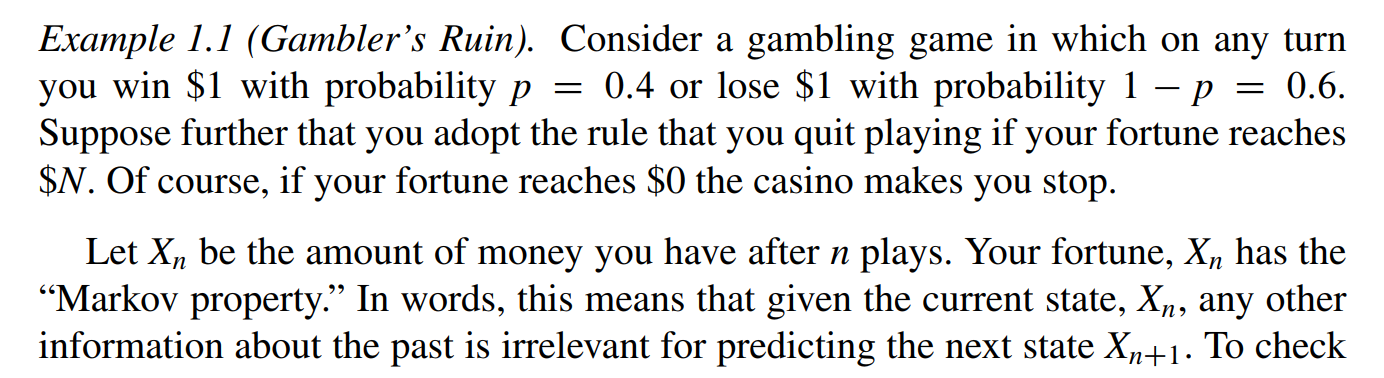
\includegraphics[width=0.9\textwidth]{figures/Gambler's Ruin.png}
        \caption{Gambler's Ruin}
    \end{figure}
\end{example}

\begin{claim}
$\{X_n,n\geq 0\}$ 为(时齐)马氏链
\end{claim}

1. 对于 $0<i_0,\cdots,i_{n-1}<N, n\geq 0$ 有
\[
\begin{aligned}
    &\PP(X_{n+1}=i+1|X_n=i,X_0=i_0,\cdots,X_{n-1}=i_{n-1})\\
    =&\PP(X_{n+1}=i+1|X_n=i)=0.4=\PP(\text{第}n+1\text{次赌局赢一元})
\end{aligned}
\]
\[
\begin{aligned}
    &\PP(X_{n+1}=i-1|X_n=i,X_0=i_0,\cdots,X_{n-1}=i_{n-1})\\
    =&\PP(X_{n+1}=i-1|X_n=i)=0.6=\PP(\text{第}n+1\text{次赌局输一元})
\end{aligned}
\]

2. $\PP(X_{n+1}=0|X_n=0,X_0=i_0,\cdots,X_{n-1}=i_{n-1})=1=\PP(X_{n+1}=0|X_n=0)$

$\PP(X_{n+1}=N|X_n=N, X_0=i_0,\cdots, X_{n-1}=i_{n-1})=1=\PP(X_{n+1}=N|X_n=N)$

最后一个等号是由题目设定得到,从 $0\to 0$ 或 $N\to N$ 的概率都为1,因为游戏结束

综上,$p(i,i+1)=0.4,0<i<N, p(i,i-1)=0.6, 0<i<N, p(0,0)=p(N,N)=1$

e.g. 

\begin{figure}[H]
    \centering
    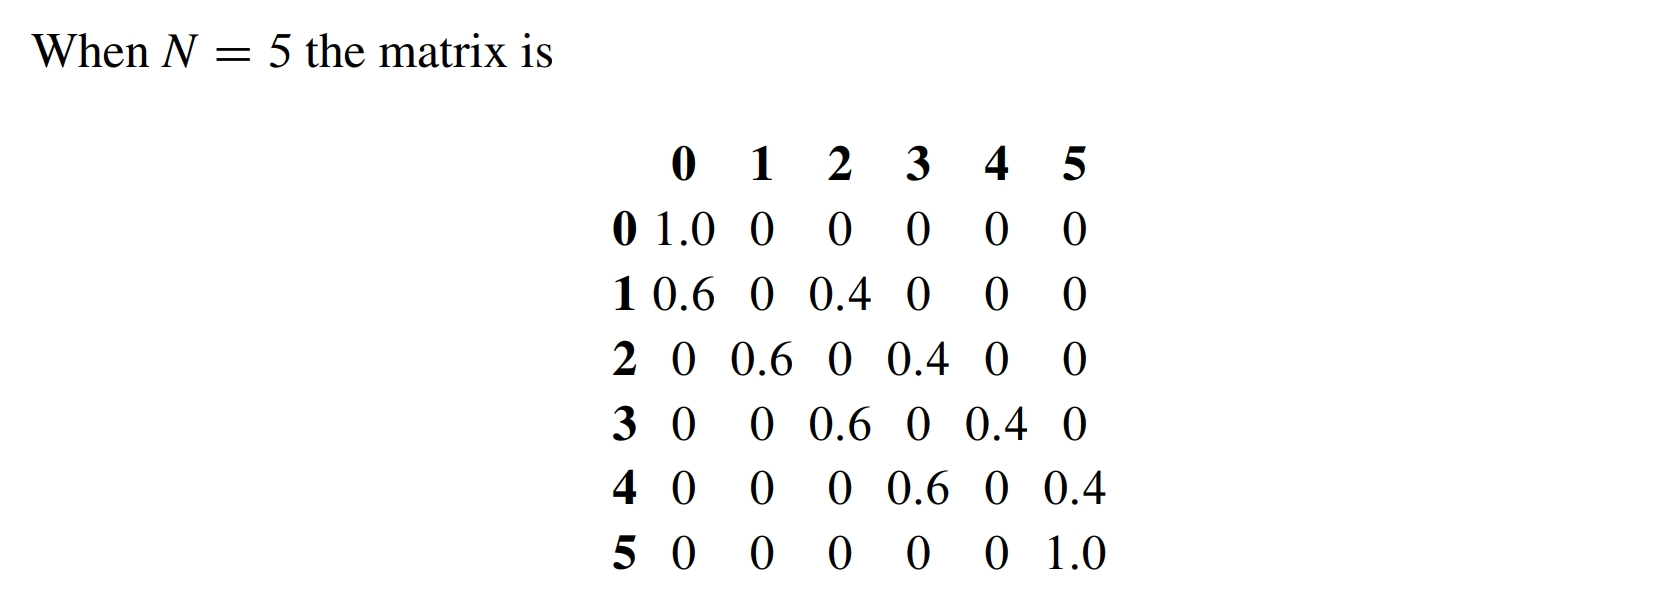
\includegraphics[width=0.9\textwidth]{figures/N=5.png}
    \caption{N=5}
\end{figure}

\begin{example}[Two-Stage Markov Chains]
    [Durrett\cite{durrett}, P7]
    \begin{figure}[H]
        \centering
        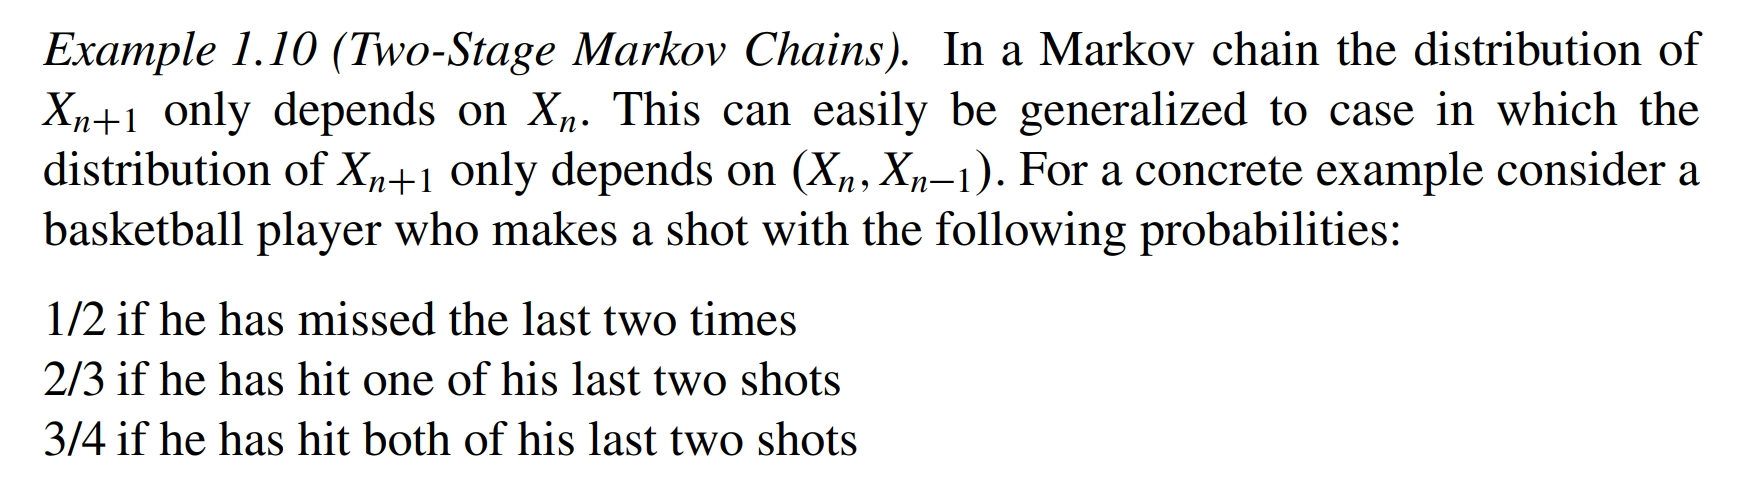
\includegraphics[width=0.9\textwidth]{figures/two_stage_markov_chains.png}
        \caption{Two-Stage Markov Chains}
    \end{figure}
\end{example}

\begin{enumerate}
    \item $\PP(X_{n+1}=H|X_n=M,X_{n-1}=M)=1/2$
    \item $\PP(X_{n+1}=H|X_n=M,X_{n-1}=H)=\PP(X_{n+1}=H|X_n=H,X_{n-1}=M)=2/3$
    \item $\PP(X_{n+1}=H|X_n=H,X_{n-1}=H)=3/4$
\end{enumerate}

\begin{claim}
$Y_n=(X_n,X_{n-1}), n\geq 1$ 则 $\{Y_n,n\geq 1\}$ 是(时齐)马氏链,$Y_n:\Omega\to \{HH,HM,MH,MM\}$ 
\end{claim}

证明:
\[
\begin{aligned}
    &\PP(Y_{n+1}=HH|Y_n=HH,Y_j=(x_j,x_{j-1}), 1\leq j\leq n-1)\\
    =& \PP(X_{n+1}=H,X_n=H|X_n=H,X_{n-1}=H,X_j=x_j,X_{j-1}=x_{j-1},0\leq j\leq n-1)\\
    =& \PP(X_{n+1}=H|X_n=H,X_{n-1}=H)\\
    =&3/4\qquad [3.]
\end{aligned}
\]

对 1.2. 同理\qed

\begin{proposition}[初见马氏链的有限维分布]\label{prop:markov_dist}
设 \(P = (p_{ij})_{i,j \in S}\) 为随机矩阵,\(\mu = (\mu_i)_{i \in S}\) 为概率分布,\(X = \{X_n, n \geq 0\}\) 为 \(S\) 值离散时间随机过程。则过程 \(X \sim \text{Markov}(\mu, P)\) 当且仅当对任意的 \(n \geq 0, i_0, i_1, \cdots, i_n \in S\),\(X\) 有有限维分布:
\begin{equation}
P(X_0 = i_0, X_1 = i_1, \cdots, X_n = i_n) = \mu_{i_0} \prod_{k=0}^{n-1} p_{i_k i_{k+1}}
\label{eq:markov_dist}
\end{equation}

\end{proposition}

证明:$\Rightarrow$ 
\[
\begin{aligned}
    &\PP(X_0=i_0,X_1=i_1,\cdots,X_n=i_n)\\
    =&\PP(X_0=i_0)\PP(X_1=i_1|X_0=i_0)\cdots \PP(X_n=i_n|X_0=i_0,\cdots X_{n-1}=i_{n-1})\quad [\text{乘法公式}\eqref{eq:multiply_func}]\\
    =&\PP(X_0=i_0)\PP(X_1=i_1|X_0=i_0)\cdots \PP(X_n=i_n|X_{n-1}=i_{n-1})\quad [\text{Markov}]\\
    =&\mu_{i_0}P_{i_0,i_1}\cdots P_{i_{n-1},i_n}
\end{aligned}
\]
严格地讲,$\PP(\cdot|A)$ 需保证 $\PP(A)>0$。对 $\PP(A)=0$ 情况的分类讨论,见 Resnick\cite{resnick}, prop 2.1.1 (\href{https://dafuzhuu.github.io/stochastic-process/pdf/Resnick.pdf}{PDF链接})

$\Leftarrow$ 

1. $n=0, \PP(X_0=i_0)=\mu_{i_0}\Rightarrow X_0\sim (\mu_i)_{i\in S}$

2. 
\[
\PP(X_{n+1}=i_{n+1}|X_0=i_0,\cdots,X_n=x_n)=\frac{\PP(X_0=i_0,\cdots,X_{n+1}=i_{n+1})}{\PP(X_0=i_0,\cdots, X_n=i_n)}=P_{i_n,i_{n+1}}
\]

由时齐马氏链定义,初始分布和转移矩阵都符合定义\ref{def:homo-markov}

\[
\therefore \quad X\sim \text{Markov}(\mu,P)
\]

对于 $\PP(X_0=i_0,X_1=i_1,\cdots,X_{n}=i_{n})$,如果我们想把 $X_1$ 挖掉,即
\[
\begin{aligned}
    \PP(X_0=i_0,X_2=i_2,\cdots,X_{n}=i_{n})&=\sum_{i_1\in S}\PP(X_0=i_0,X_1=i_1,\cdots,X_{n}=i_{n})\\
    &=\mu_{i_0}\sum_{i_1\in S}(P_{i_0,i_1}P_{i_1,i_2})\cdots P_{i_{n-1},i_n}
\end{aligned}
\]

\begin{figure}[H]
    \centering
    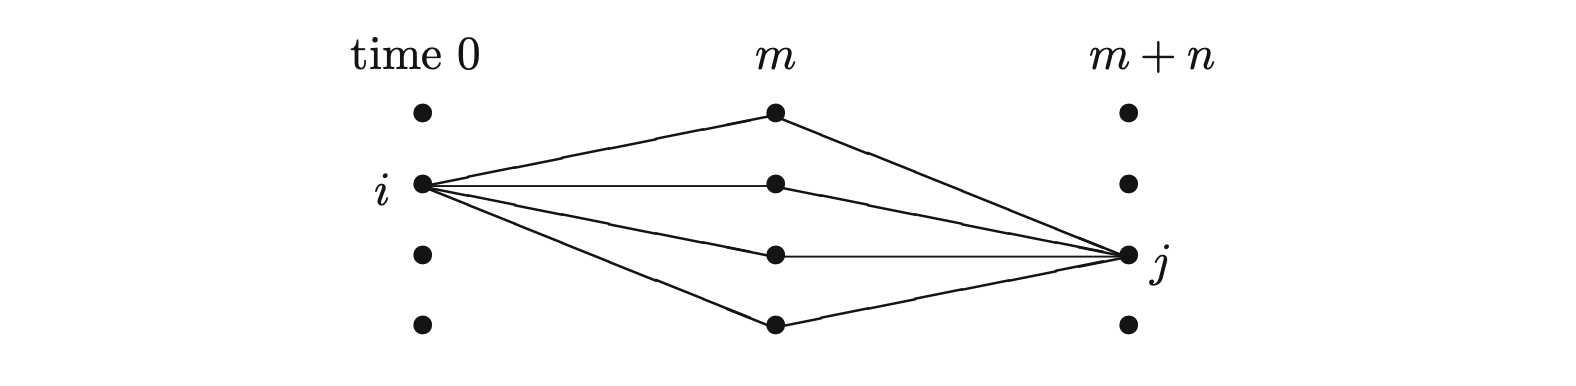
\includegraphics[width=0.9\textwidth]{figures/split_steps.png}
\end{figure}

\subsection{多步转移概率与矩阵乘法}

\begin{definition}
    设 $X=\{X_n,n\geq 0\}$ 为马氏链,称
    \[
    p_{ij}(m,m+n):=\PP(X_{n+m}=j|X_m=i)\quad (i,j\in S, m,n\geq 0)
    \]
    为 $X$ 的 $n$ 步转移概率,并称 $P(m,m+n)=(p_{ij}(m,m+n))_{i,j\in S}$ 为 $X$ 的 $n$ 步转移(概率)矩阵,其中
    \[
    p_{i,j}(0,0)=\delta_{ij}=\begin{cases}
        1 & i=j\\
        0 & i\neq j
    \end{cases}
    \]
\end{definition}

当 $X$ 时齐,$P(m,m+1)=(p_{ij}(m,m+1))_{i,j\in S}=(p_{ij}(0,1))_{i,j\in S}=(p_{ij})_{i,j\in S}$

可见 $n=1$ 时,$P(m,m+1)$ 与 $m$ 无关。那 $n>1$ 时呢?

\subsubsection{Chapman-Kolmogorov方程}

\begin{theorem}[C-K方程]\label{thm:CK}
    设 $\{X_n,x\geq 0\}$ 为马氏链
    \[
    p_{ij}(m,m+n+r)=\sum_{k\in S}p_{ik}(m,m+n)p_{kj}(m+n,m+n+r)
    \]
    其中 $i,j\in S,m,n,r\geq 0$,即
    \[
    P(m,m+n+r)=P(m,m+n)P(m+n,m+n+r)
    \]
\end{theorem}

\begin{figure}[H]
    \centering
    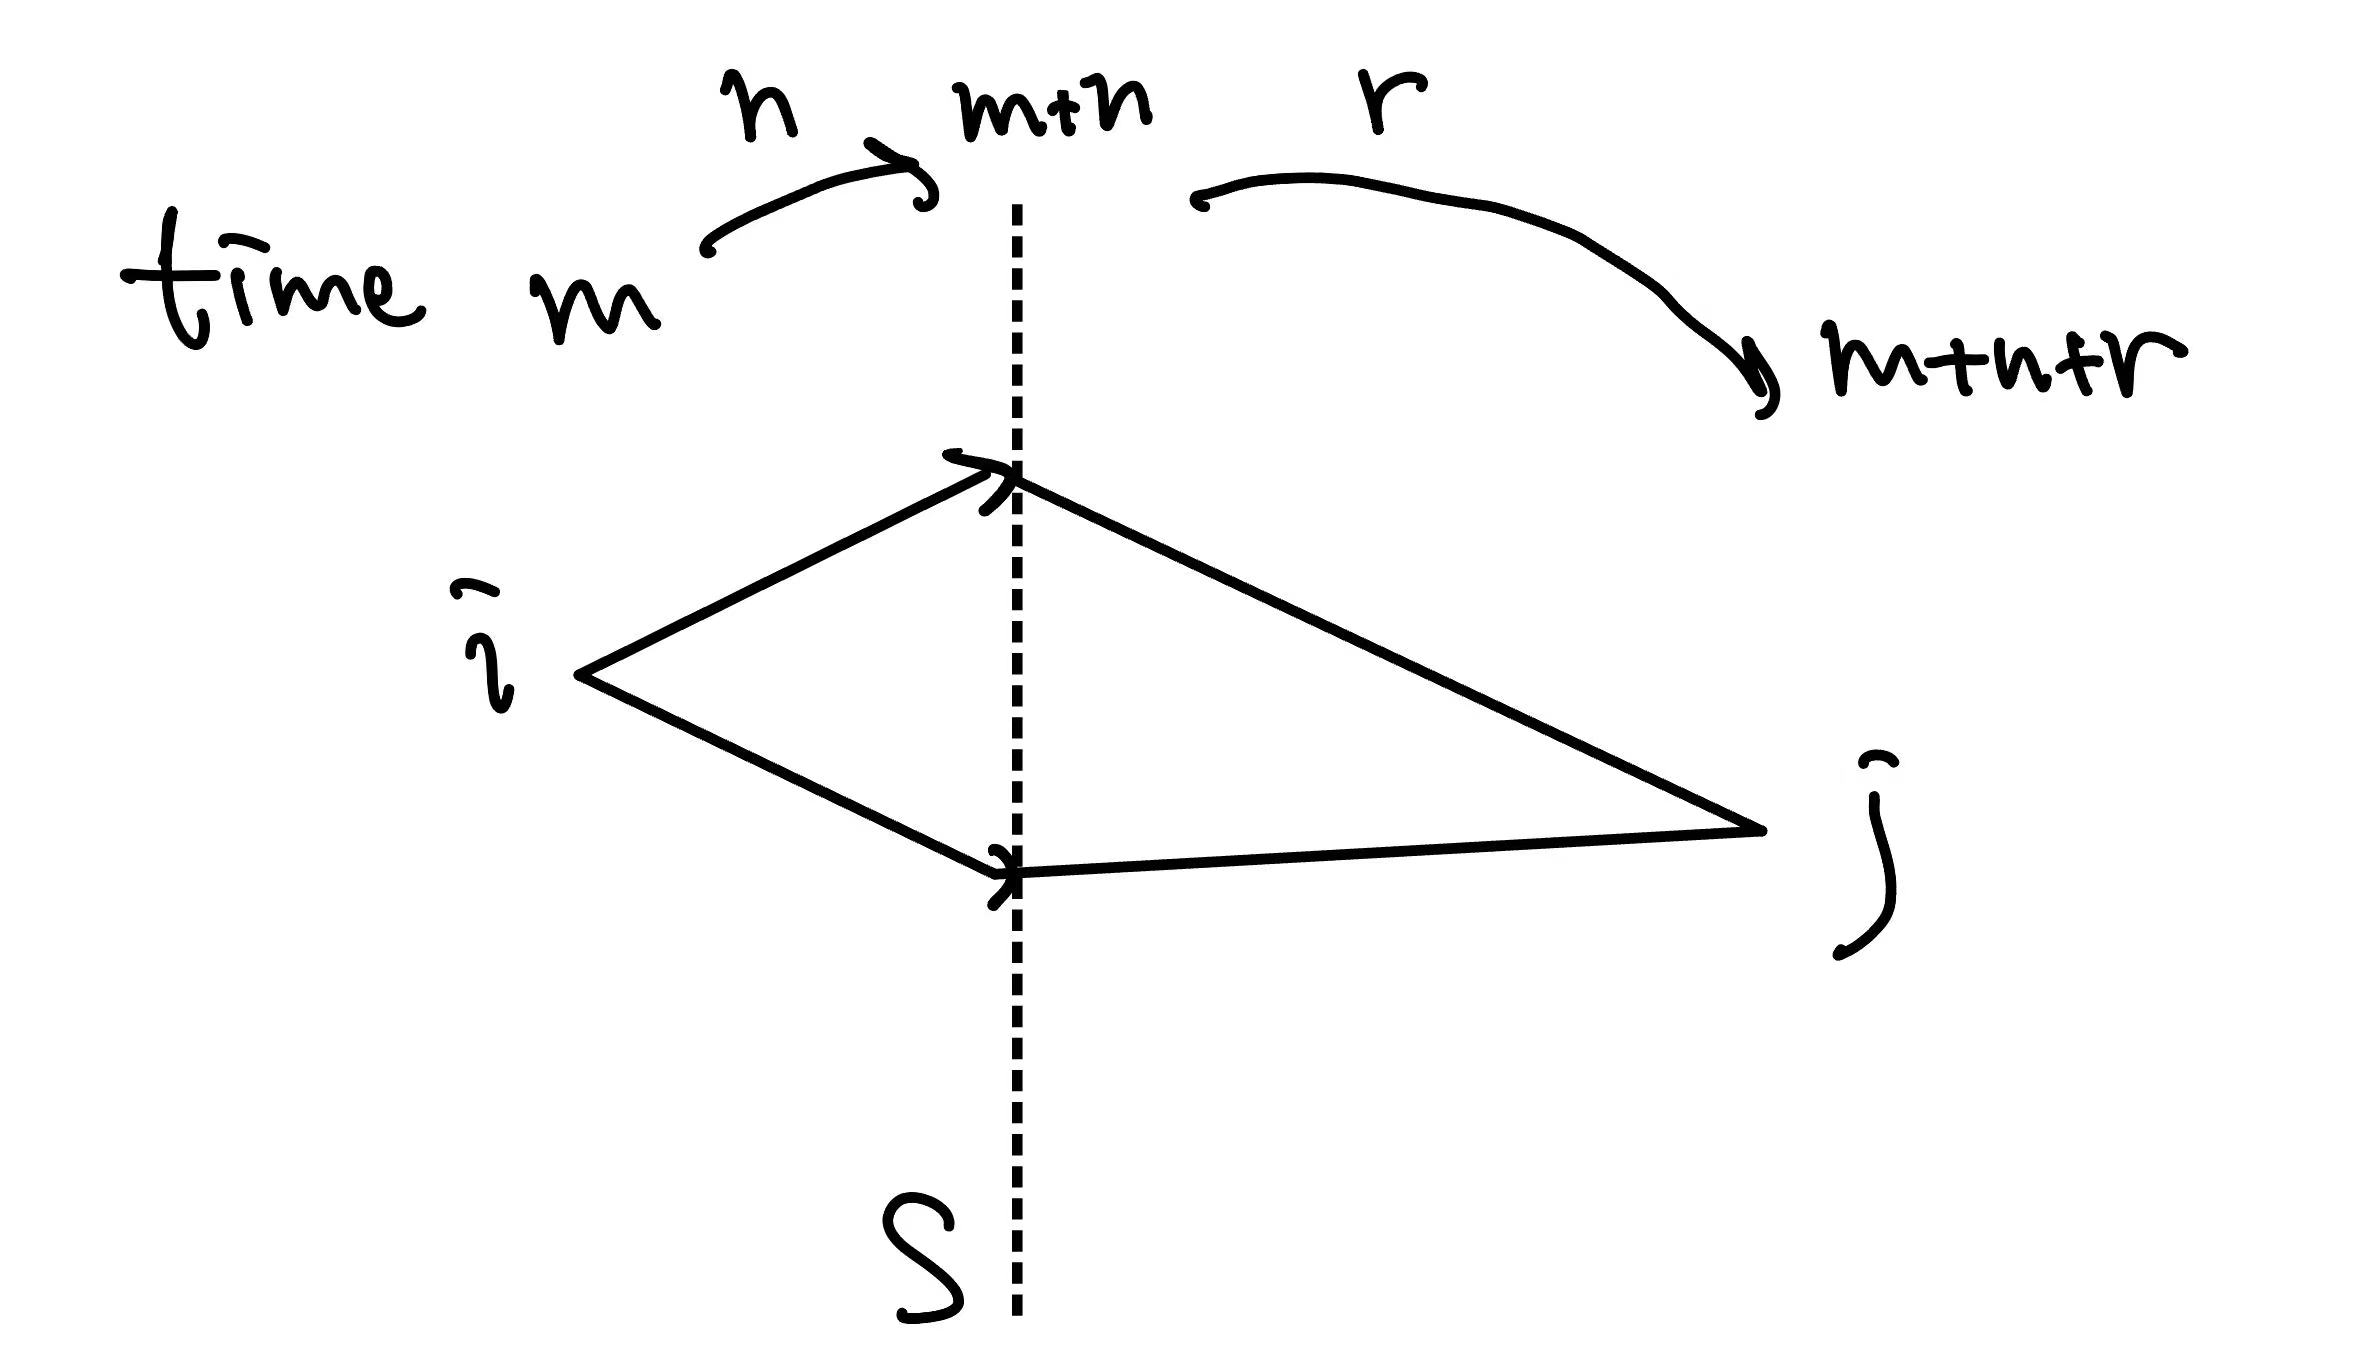
\includegraphics[width=0.55\textwidth]{figures/multi_steps.jpg}
    \caption{Multi-steps}
\end{figure}

证明:

\[
\begin{aligned}
    p_{ij}(m,m+n+r)&=P(X_{m+n+r}=j|X_m=i)\\
    &=\sum_{k\in S}P(X_{m+n+r}=j,X_{m+n}=k|X_m=i)\\
    &=\sum_{k\in S}\PP_{\{X_m=i\}}(X_{m+n+r}=j|X_{m+n}=k)\PP_{\{X_m=i\}}(X_{m+n}=k)\quad [\text{乘法公式}\eqref{eq:multiply_func}]\\
    &=\sum_{k\in S}p_{ik}(m,m+n)p_{kj}(m+n,m+n+r)\quad [\text{Markov}]
\end{aligned}
\]

\begin{corollary}
    设 $X$ 为具有(一步)转移矩阵 $P$ 的时齐马氏链,则
    \begin{enumerate}
        \item $\forall m,n\geq 0$,有 $P(m,m+n)=P(0,n)=P^n$。其中,约定 $P^0=I$(单位矩阵)
        
        从而,可记 $X$ 的 $n$ 步转移概率为 $p_{ij}(n)$ 或 $p_{ij}^{(n)}$,$n$ 步转移概率矩阵为 $P(n)$,且有
        \[
        P(n)=P^n=(p_{ij}^{(n)})_{i,j\in S}
        \]
        \item C-K 方程可改写为
        \[
        p_{ij}(m+n)=\sum_{k\in S}p_{ik}^{(m)}p_{kj}^{(n)}
        \]
        $P(m+n)=P(m)P(n)$,即 $P^{m+n}=P^m P^n$
    \end{enumerate}
\end{corollary}

证明:

\[
\begin{aligned}
    P(m,m+n)&=P(m,m+1)\cdot P(m+1,m+n)\quad [\text{C-K}]\\
    &=P\cdot P(m+1,m+n)\quad [\text{时齐}]\\
    &=P^n\qed
\end{aligned}
\]

\begin{proposition}
    $\forall n\geq 0, P(n)=P^n$ 仍是一个随机矩阵(定理\ref{thm:random_matrix})
\end{proposition}

证明:$n=2$时,$P^2=(p_{ij}(2))_{i,j\in S}$

$\Rightarrow$
\[
\begin{aligned}
    \sum_{j\in S}p_{ij}(2)&=\sum_{j\in S}\sum_{k\in S}p_{ik}p_{kj}\quad [\text{C-K}, \text{ 默认}p_{ik}(1)=p_{ik}]\\
    &=\sum_{k\in S}\sum_{j\in S}p_{ik}p_{kj}\\
    &=\sum_{k\in S}p_{ik}\cdot(\sum_{j\in S}p_{kj})\\
    &=\sum_{k\in S}p_{ik}=1\qed
\end{aligned}
\]
第二个等号,级数可交换是因为非负,要么有限(收敛)、要么$+\infty$(发散)

\subsubsection{马氏链的任意有限维分布}

\begin{proposition}
    $X\sim\text{Markov}(\mu, P)$,其中 $\mu=(\mu_i)_{i\in S}, P=(p_{ij})_{i,j\in S}$,则
    \[
    \PP(X_{u_1}=i_1,\cdots,X_{u_n}=i_n)=\mu_{i_1}^{(u_1)}\prod_{k=1}^{n-1}p_{i_k,i_{k+1}}^{(u_{k+1}-u_k)}
    \]
    其中,$0<u_1<u_2<\cdots<u_n$,$i_1,i_2,\cdots,i_n\in S$,$\mu^{(u_1)}=(\mu_i^{(u_1)})_{i\in S}$ 为 $X_{u_1}$ 的有限维分布
\end{proposition}

证明:
\[
\begin{aligned}
    \PP(X_{u_1}=i_1,\cdots,X_{u_n}=i_n)&=\PP(X_{u_1}=i_1)\cdot \PP(X_{u_2}=i_2|X_{u_1}=i_1)\cdots \PP(X_{u_n}=i_n|X_{u_1}=i_1,\cdots,X_{u_{n-1}}=i_{n-1})\\
    &=(\mu_{i_1}^{(u_1)})p_{i_1,i_2}^{(u_2-u_1)}\cdots p_{i_{n-1},i_n}^{(u_n-u_{n-1})}\quad [\text{Markov}]\\
    &=\mu_{i_1}^{(u_1)}\prod_{k=1}^{n-1}p_{i_k,i_{k+1}}^{(u_{k+1}-u_k)}
\end{aligned}
\]

用概率表示不够直观,尝试用转移矩阵来表示

\begin{lemma}
   $\mu^{(m+n)}=\mu^{(n)}P^m(\forall m,n\geq 0)$,即
   \[
   \mu_j^{(m+n)}=(\mu^{(n)}P^m)_j=\sum_{i\in S}\mu_i^{(n)}p_{ij}^{(m)}
   \]
   特别地,取 $n=0$,则 $\mu^{(m)}=\mu\cdot P^m$($\mu$看成行向量),即 $\mu_j^{(m)}=(\mu P^m)_j=\sum_{i\in S}\mu_i\cdot p_{ij}^{(m)}$
\end{lemma}

证明:
\[
\begin{aligned}
    \mu_j^{(n+m)}=\PP(X_{n+m}=j)&=\sum_{i\in S}\PP(X_{n+m}=j|X_n=i)\PP(X_n=i)\\
    &=\sum_{i\in S}p_{ij}(m)\mu_i^{(n)}\\
    &=(\mu^{(n)}P^m)_j\qed
\end{aligned}
\]

$\Rightarrow \mu^{(m+n)}=\mu^{(n)}P^m$

\begin{theorem}[任意有限维分布II]
    $\forall 0\leq u_1<u_2<\cdots<u_n, i_1,\cdots,i_n\in S$
    \[
    \PP(X_{u_1}=i_1,\cdots,X_{u_n}=i_n)=(\mu P^{u_1})_{i_1}\prod_{k=1}^{n-1}P_{i_k,i_{k+1}}^{u_{k+1}-u_k}
    \]
    其中,$P_{i,j}^m=:(P^m)_{i,j}=:p_{i,j}^{(m)}$
\end{theorem}

讨论随机过程地存在性:

抽象地,$\mu,P\xrightarrow{\text{定理}\eqref{thm:Kolmogorov}}\text{有限维分布族}\rightarrow X\sim \text{Markov}(\mu,P)$,$\mu,P$可以刻画具备对称性、相容性的有限维分布

具体地,参考Resnick\cite{resnick}, P62, Section 2.1 (\href{https://dafuzhuu.github.io/stochastic-process/pdf/Resnick.pdf}{PDF链接})

\subsection{(从固定点出发的)马氏链}

固定 $i\in S$,定义 $\PP_i(\cdot)=\PP(\cdot|X_0=i)$, $\EE_i(X)=\EE(X|X_0=i)=\sum_{x\in S}x\PP_i(X=x)$

\subsubsection{链的状态:常返和暂留}

\begin{definition}
    称状态 $i$ 为常返的,若
    \[
    \PP_i(X_n=i\text{对某个}n\geq 1)=1
    \]
    如果上面的概率$<1$,则称为暂留的/非常返的
\end{definition}

注:$i$ 常返 $\Leftrightarrow$ $\PP_i(\cup_{n\geq 1}\{X_n=i\})=1$

思考:$i$ 常返 $\Leftrightarrow$ “不停地/无数次回到$i$”

$\qquad \Leftrightarrow$ $\PP_i(\omega|\omega\in \text{无数多个} \{X_n=i\})$

$\qquad \Leftrightarrow$ $\PP_i(\omega|\omega\in\cap_{k\geq 1}\cup_{n\geq k}\{X_n=i\},\forall k)$

$\qquad \Leftrightarrow$ $\PP_i(X_n=i, i.o.)$ (infinitely often)

无数多次返回 $i$ 可严格定义为:
\[
\bigcap_{k\geq 1}\bigcup_{n\geq k}\{X_n=i\}
\]
集合的语言中,$\cup$即$\exists$,$\cap$即$\forall$,因此
\begin{itemize}
    \item $\bigcup_{n\geq k}\{X_n=i\}$ 表示 $\exists n_0\geq k$ 使得 $X_{n_0}=i$
    \item 对 $\forall k$ 取交集 $\bigcap_{k\geq 1}$,即无论 $k$ 多大,总存在更大的 $n$ 满足 $X_n=i$,从而保证无限次返回
\end{itemize}
即 $\forall k, \exists n_k, s.t. \{X_{n_k}=i\}$发生
\[
\begin{aligned}
    k=1&, n_1\geq k\\
    k=n_1+1&, n_2\geq n_1+1>n_1\\
    &\cdots
\end{aligned}
\]

\begin{remark}[如何进一步理解]
    无界和$\infty$的区别是什么?

无界:$\forall M>0,\exists k, s.t. |x_k|>M$
\begin{example}
    $1,2,3,4,\cdots$ 为 $\infty$/无界

    $1,0,2,0,3,0,4,\cdots$ 并非 $\infty$,但是无界的
\end{example}
迁移到$\bigcap_{k\geq 1}\bigcup_{n\geq k}$的例子
\begin{example}
    $A_1=\{0,1\},A_2=\{2\},A_3=\{0,3\},\cdots$,则
    \[
    \bigcap_{k=1}^{\infty}\bigcup_{n\geq k}A_n=\{0\},\qquad \bigcap_{k=1}^{\infty}A_k=\emp
    \]
    其中 $\bigcap_{k=1}^{\infty}\bigcup_{n\geq k}$ 也即 $\limsup$
\end{example}
\end{remark}

但我们推理得到的“常返”和定义里的并不等价
\[
\bigcap_{k\geq 1}\bigcup_{n\geq k}\{X_n=i\}\nLeftrightarrow \bigcup_{n\geq 1}\{X_n=i\}
\]
且LHS是RHS的子集,因此由定义的$\PP(RHS)=1$不能推出$\PP(LHS)=1$。于是我们疑惑为什么会叫它常返。这里要用到高阶知识“停时”,我们最后会回到这个问题。

下面给出几种判断常返/暂留的方法。

\subsubsection{从数学角度:并改写成不交并}

$i$ 常返 $\Leftrightarrow$ $\PP_i(\cup_{n\geq 1}\{X_n=i\})=1$

$\qquad \Leftrightarrow \PP_i(\text{有限步到达}i)=1$

$\qquad \Leftrightarrow \PP(\text{从}i\text{出发条件下,有限时间内回到}i)=1$

$B_1(i)=\{X_1=i\},B_2(i)=\{X_2=i\}\backslash \{X_1=i\}=\{X_2=i,X_1\neq i\},$ $\cdots,$ $B_n(i)=\{X_n=i,X_{n-1}\neq i\cdots,X_1\neq i\}$
\[
\Rightarrow\quad \sum_{n\geq 1}B_n(i)=\bigcup_{n\geq 1}\{X_n=i\} [\text{练习}\eqref{exer:disjoint_union}]
\]
$i$ 常返 $\Leftrightarrow$ $1=\PP_i(\sum_{n\geq 1}B_n(i))=\sum_{n\geq 1}\PP_i(B_n(i))$,第二个等号由可列可加性得到(定义\ref{def:prob_measure})
\[
\begin{aligned}
    \PP_i(B_n(j))&=\PP_i(X_n=j,X_{n-1}\neq j,\cdots,X_1\neq j)\\
    &=\PP_i(\text{首次访问}j\text{的时刻为}n)\\
    &=\PP_i(\text{走}n\text{步首次到达}j)
\end{aligned}
\]
故
\[
\begin{aligned}
    \PP_i(\sum_{n\geq 1}B_n(i))&=\PP_i(\text{首次访问}j\text{的时刻为有限时间})\\
    &=\PP_i(\text{有限时间内首次访问}j)
\end{aligned}
\]
记号
\[
f_{ij}:=\PP_i(\text{首次访问}j\text{的时刻为有限时间})
\]
\[
f_{ij}(n):=\PP_i(B_n(j))=\PP_i(\text{首次访问}j\text{的时刻为}n)
\]

\begin{proposition}
    常返和暂留的等价命题
    \begin{enumerate}
        \item $i$ 常返 $\Leftrightarrow$ $1=f_{ii}=\sum_{n\geq 1}f_{ii}(n)$
        \item $i$ 暂留 $\Leftrightarrow$ $1>f_{ii}=\sum_{n\geq 1}f_{ii}(n)$
    \end{enumerate}
\end{proposition}

\subsubsection{从“多步转移概率”角度判别}

定义新记号($P$不是转移矩阵)
\[
P_{ij}(s):=\sum_{n\geq 0}s^n p_{ij}(n)\qquad F_{ij}(s):=\sum_{n\geq 0}s^n f_{ij}(n)
\]
其中,$p_{ij}(0)=\delta_{ij},f_{ij}(0)=0$
\[
\delta_{ij}=\begin{cases}
    1 & i=j\\
    0 & i\neq j
\end{cases}
\]

注:当 $|s|<1$ 时,$P_{ij}(s),F_{ij}(s)$ 绝对收敛

由 Abel 连续性定理,
\[
\lim_{s\uparrow 1}F_{ij}(s)=\sum_{n\geq 1}f_{ij}(n)=f_{ij}\in [0,1]
\]
\[
\lim_{s\uparrow 1}P_{ij}(s)=\sum_{n\geq 0}p_{ij}(0)=\text{finite}/+\infty
\]
\begin{lemma}
    [Grimmett\cite{grimmett}, Thm 6.3.3] 设 $|s|<1$,则
    \[
    P_{ij}(s)=\delta_{ij}+P_{jj}(s)F_{ij}(s)
    \]
    其中
    \[
    \delta_{ij}=\begin{cases}
        1 & i=j\\
        0 & i\neq j
    \end{cases}
    \]
\end{lemma}

证明:构造不交并,$B_m(i)=\{X_m=i,X_{m-1}\neq i,\cdots,X_1\neq i\}, m\geq 1$

$\Rightarrow$ $\sum_{m\geq 1}B_m(i)=\cup_{n\geq 1}\{X_n=i\}, B_m(i)\st \{X_n\neq i\}, m\geq n+1$
\[
\begin{aligned}
    p_{ij}(n)=\PP_i(X_n=j)&=\PP_i(\{X_n=j\}\cap \sum_{m\geq 1}B_m(j))\\
    &=\sum_{m\geq 1}\PP_i(\{X_n=j\}\cap B_m(j))
    &=\sum_{m=1}^n\PP_i(\{X_n=j\}\cap B_m(j))
\end{aligned}
\]
最后一个等号成立是因为 $m\geq n+1$ 时 $\{X_n=j\}\cap B_m(j)$ 为空集
\[
\sum_{m=1}^n\PP_i(\{X_n=j\}\cap B_m(j))=\sum_{m=1}^n\PP_i(X_n=j|B_m(j))\PP_i(B_m(j))
\]
其中 $X_m=j,X_{n-1}\neq j,\cdots,X_1\neq j$,$X_{n-1}\in S\backslash \{j\}$

用一般而非单点的马氏性(引理\ref{lem:markov_equiv}$M_3$)
\[
\begin{aligned}
    \sum_{m=1}^n\PP_i(X_n=j|B_m(j))\PP_i(B_m(j))&=\sum_{m=1}^n\PP(X_n=j|X_m=j)\cdot f_{ij}(m)\\
    &=\sum_{m=1}^n p_{jj}(n-m)\cdot f_{ij}(m)
\end{aligned}
\]
当 $n\geq 1$ 时,
\[
\begin{aligned}
    P_{ij}(s)&=s^0p_{ij}(0)+\sum_{n\geq 1}s^n\cdot p_{ij}(n)\\
    &=\delta_{ij}+\sum_{n\geq 1}s^n\sum_{m=1}^n p_{jj}(n-m)f_{ij}(m)\\
    &=\delta_{ij}+\sum_{n\geq 1}\sum_{m=1}^n s^n p_{jj}(n-m)f_{ij}(m)\\
    &=\delta_{ij}+\sum_{n\geq 1}\sum_{m=1}^n(s^{n-m}p_{jj}(n-m))(s^m f_{ij}(m))\\
    &=\delta_{ij}+\sum_{n=1}^{\infty}\sum_{m=1}^{\infty}\II_{\{1\leq m\leq n\}}(s^{n-m}p_{jj}(n-m))(s^m f_{ij}(m))
\end{aligned}
\]
把 $\II_{\{1\leq m\leq n\}}(s^{n-m}p_{jj}(n-m))(s^m f_{ij}(m))$ 看作 $a_{n,m}$,由推论\ref{lem:abs_convergence}考察绝对收敛

$0\leq s<1, |s|=s$

正向级数一定有意义,就看是有限/$\infty$
\[
\begin{aligned}
    &\sum_{n=1}^{\infty}\sum_{m=1}^{\infty}\II_{\{1\leq m\leq n\}}s^{n-m}p_{jj}(n-m)s^m f_{ij}(m)\\
    =&\sum_{m=1}^{\infty}\sum_{n=1}^{\infty}\II_{\{1\leq m\leq n\}}s^{n-m}p_{jj}(n-m)s^m f_{ij}(m)\\
    =&\sum_{m=1}^{\infty}(\sum_{n=m}^{\infty}s^{n-m}p_{jj}(n-m))s^m f_{ij}(m)\\
    =&(\sum_{n=0}^{\infty}s^{n}p_{jj}(n))(\sum_{m=1}^{\infty}s^m f_{ij}(m))<\infty\quad [\text{变量代换}n\leftarrow n-m]
\end{aligned}
\]
因为 $s^0f_{ij}(0)=0$,则 $\sum_{m=0}^{\infty}s^m f_{ij}(m)=\sum_{m=1}^{\infty}s^m f_{ij}(m)$。代回原式
\[
P_{ij}(s)=\delta_{ij}+P_{jj}(s)\cdot F_{ij}(s)
\]

\begin{proposition}\label{prop:states_equiv}
    (1) $j$ 常返 $\Leftrightarrow$
    \[
        1=f_{jj}\Leftrightarrow \sum_{n\geq 0}p_{jj}(n)=\infty
    \]
    (2) $j$ 暂留 $\Leftrightarrow$
    \[
    \begin{aligned}
        1>f_{jj}&\Leftrightarrow \sum_{n\geq 0}p_{jj}(n)<\infty\\
        &\Rightarrow \sum_{n\geq 0}p_{ij}(n)<\infty, \forall i\in S\\
        &\Rightarrow \limit{n}p_{ij}(n)=0,\forall i\in S
    \end{aligned}
    \]
\end{proposition}

证明:只证(1). $|s|<1$时,$P_{ij}(s)=\delta_{ij}+P_{jj}(s)F_{ij}(s)$

$\Rightarrow P_{jj}(s)=1+P_{jj}(s)F_{jj}(s)$

$\Rightarrow$
\[
P_{jj}(s)=\frac{1}{1-F_{jj}(s)}\tag{*}
\]
$j$ 常返 $\Leftrightarrow$ $1=f_{jj}=F_{jj}(1)\overset{\text{Abel}}{=}\lim_{s\uparrow 1}F_{jj}(s)$

对 (*),令 $s\to 1$,有 $\sum_{n\geq 0}p_{jj}(n)=+\infty$

\begin{problem}[作业5-1]
证明:$j$ 暂留 $\Rightarrow \sum_{n\geq 0}p_{ij}(n)<\infty, \forall i\in S$
\end{problem}

\subsubsection{从“首次回访时间”角度判别}
\[
\begin{aligned}
    j\text{常返}&\Leftrightarrow 1=\PP_j(X_n=j\text{ 对某个}n\geq 1)=\PP_j(\text{有限时间内回访}j)\\
    &\Leftrightarrow 1=f_{jj}=\PP_j(\underbrace{\text{首次回访}j\text{的时刻}}_{T_j<\infty}\text{有限})\\
    &\quad =\sum_{n\geq 1}f_{jj}(n)=\sum_{n\geq 1}\PP_j(\underbrace{\text{首次回访}j\text{的时刻}}_{T_j=n}\text{是}n)
\end{aligned}
\]
\begin{definition}
    首次回访$j$的时刻
    \[
    T_j=\min\{n\geq 1|X_n=j\}
    \]
    约定 $\min \emp=+\infty$
\end{definition}

注:$\{T_j=\infty\}\Leftrightarrow \{\omega|\{n\geq 1|X_n(\omega)=j\}=\emp\}$

$\quad \Leftrightarrow \{\omega|X_n(\omega)\neq j,\forall n\geq 1\}=\cap_{n\geq 1}\{X_n\neq j\}$

\begin{property}
    $f_{jj}=\PP_j(T_j<\infty), f_{jj}(n)=\PP_j(T_j=n)$
\end{property}

定义 $\PP_j(T_j<\infty)=\rho_{jj}$

\begin{proposition}
    联系命题\ref{prop:states_equiv}
    \begin{enumerate}
        \item $j$ 常返 $\Leftrightarrow$ $1=\rho_{jj}=\PP_j(T_j<\infty)\Leftrightarrow 0=\PP_j(T_j=\infty)$
        \item $j$ 暂留 $\Leftrightarrow$ $1>\rho_{jj}=\PP_j(T_j<\infty)\Leftrightarrow 0<\PP_j(T_j=\infty)$
    \end{enumerate}
\end{proposition}

\begin{definition}
    $j$ 的平均回访时间
    \[
    m_j:=\EE_jT_j=\EE(T_j|X_0=j)
    \]
\end{definition}

\begin{theorem}
    \[
    m_j=\EE_j T_j=\begin{cases}
        \sum_{n\geq 1}nf_{jj}(n) & j\text{常返}\\
        \infty & j\text{暂留}
    \end{cases}
    \]
\end{theorem}

证明:

(1) $j$暂留 $\Rightarrow$ $\PP_j(T_j=\infty)>0$

$\quad \Rightarrow \EE T_j=\EE T_j\II_{\{T_j=\infty\}}+\EE T_j\II_{\{T_j<\infty\}}\geq \EE T_j\II_{\{T_j=\infty\}}=\infty\cdot \PP_{T_j=\infty}=\infty$

(2) $j$常返 $\Rightarrow$ $\PP_j(T_j=\infty)=0$

取期望时不起作用,因为 $0\cdot \infty$ 是不定形
\[
\begin{aligned}
    \EE_j T_j&=\EE_j T_j\II_{\{T_j<\infty\}}\\
    &=\EE_j T_j\II_{\sum_{n\geq 1}\{T_j=n\}}\\
    &=\EE_j\sum_{n\geq 1}T_j\II_{\{T_j=n\}}\quad [\text{定义\eqref{def:discrete_rv}}]\\
    &=\sum_{n\geq 1}n\PP_j(T_j=n)\\
    &=\sum_{n\geq 1}n f_{jj}(n)
\end{aligned}
\]
\begin{definition}
    $j$常返时
    \begin{enumerate}
        \item $\EE_j T_j<\infty$ 称$j$是正常返
        \item $\EE_j T_j=\infty$ 称$j$是零常返(平均意义上再也不回来)
    \end{enumerate}
\end{definition}

$j$ 常返 $\Leftrightarrow 1=f_{jj}\Leftrightarrow \sum_{n\geq 0}p_{jj}(n)=\infty$

$\Leftrightarrow 1=\rho_{jj}=\PP_j(T_j<\infty)\Leftrightarrow 0=\PP_j(T_j=\infty)$
\[
\begin{aligned}
    \PP_j(T_j<\infty)&=\PP(\text{从}j\text{出发条件下,首次回到}j\text{的时刻有限})\\
    &=\PP(\text{从}j\text{出发条件下,有限时间内至少访问}j\text{有1次})\\
    &=\PP(\text{从}j\text{出发条件下,有限时间内回访}j\text{的次数}\geq 1)
\end{aligned}
\]

\begin{definition}
    链在时刻$0$之后,访问$j$的次数
    \[
    N(j):=\# \{n\geq 1|X_n=j\}=\sum_{n\geq 1}\II_{X_n=j}
    \]
\end{definition}

注:$N(j):\Omega\to \{0,1,2,\cdots\}\cup \{+\infty\}$

至此,做个阶段性小结,回顾 $i$ 常返的几种等价表示
\[
\begin{aligned}
    i\text{常返} &\overset{\text{Def}}{\Leftrightarrow}1=\PP_i(\bigcup_{n\geq 1}\{X_n=i\})\\
    &\Leftrightarrow 1=f_{ii}:=\sum_{n\geq 1}f_{ii}(n)=\sum_{n\geq 1}\PP_i(X_1\neq i,\cdots, X_{n-1}\neq i,X_n=i)\Leftrightarrow \sum_{n\geq 1}p_{ii}(n)=\infty\\
    &\Leftrightarrow 1=\rho_{ii}=\PP_i(T_i^{(1)}:=T_i<\infty)=\PP_i\{N(i)\geq 1\}=1
\end{aligned}
\]

无数次地回访 $\leftrightarrow$ 访问次数$=\infty$ $\leftrightarrow$ $\PP_i(N(i):=\sum_{n\geq 1}\II_{\{X_n=i\}}=\infty)=1$

两种表述的等价条件互相等价吗?即
\[
\PP_i(N(i)\geq 1)\overset{?}{\Leftrightarrow} \PP_i(N(i)=\infty)=1
\]
需要 Strong Markov Property (SMP) 使上面$\Leftrightarrow$成立。这里先补充一些关于 $N(j)$ 的内容,然后再回到证明。

考察 $\{N(y)=\infty\}=\cap_{k\geq 1}\{N(y)\geq k\}$

由概率测度的连续性(性质\ref{prt:measure_continuity})
\[
    \PP_x(N(y)=\infty)=\limit{k}\PP_x(N(y)\geq k)
\]
其中,
\[
\begin{aligned}
    \PP_x(N(y)\geq k) &= \PP(\text{从}x\text{出发条件下,访问}y\text{的次数}\geq k)\\
    &=\PP(\text{从}x\text{出发条件下,至少访问}y\text{有}k\text{次})\\
    &=\PP(\text{从}x\text{出发条件下,第}k\text{次访问}y\text{的时刻有限})
\end{aligned}
\]
$T_y^{(1)}:=T_y:=\min\{n\geq 1|X_n=y\}$

$T_y^{(2)}:=\min\{n>T_y^{(1)}|X_n=y\}$

$\quad \vdots$

$T_y^{(k)}:=\min\{n>T_y^{(k-1)}|X_n=y\}, \forall k\geq 2$
\[
\Rightarrow \quad \PP_x(N(y)\geq k)=\PP_x(T_y^{(k)}<\infty)
\]

\begin{definition}
    第$k$次访问概率
    \[
    \rho_{xy}^{(k)}:=\PP_x(T_y^{(k)}<\infty)
    \]
    其中,$\rho_{xy}^{(1)}=\rho_{xy}$
    
    第$k$次回访概率
    \[
    \rho_{yy}^{(k)}:=\PP_y(T_y^{(k)}<\infty)
    \]
\end{definition}

注:$\rho_{yy}^{(2)}\overset{?}{=}\rho_{yy}\cdot \rho_{yy}$

直观上是这样,但严格证明要求SMP

这是因为不同时间对应的是不同的随机过程,如
\begin{itemize}
    \item $t=0$时,过程是$\{X_n,n\geq 0\}$
    \item $t=T_j$时,过程是$\{X_{T_j+n},n\geq 0\}$
\end{itemize}
SMP是一个使得 $X_{T_j+n}=X_n,\forall T_j$ 的性质,之后会详细说。以上结论可总结成下面引理。

\begin{lemma}
    (由SMP知) $\rho_{xy}^{(k)}=\rho_{xy}\rho_{yy}^{(k-1)}$

    特别地,$\rho_{yy}^{(k)}=\rho_{yy}^k$
\end{lemma}

接着我们回到证明
\[
    \PP_i(N(i)\geq 1)=1 \Leftrightarrow \PP_i(N(i)=\infty)=1
\]

证明:$\Leftarrow$ 显然,因为 $\{N(i)=\infty\}$ 相对 $N(i)\geq 1$ 是小集合

$\Rightarrow$
\[
\PP_i(N(i)=\infty)=\limit{k}\PP_i(N(i)\geq k)\overset{\text{SMP}}{=}\limit{k}\rho_{ii}^k=1
\]
暂留的证明同理:
\[
\begin{aligned}
    i\text{暂留}&\Leftrightarrow \PP_i(N(i)=\infty)=\limit{k}\rho_{ii}^k=0\\
    &\Leftrightarrow 1> \rho_{ii}
\end{aligned}
\]

\subsubsection{从“平均回访次数”角度判别}

\[
N(y)=\sum_{n\geq 1}\II_{\{X_n=y\}}=\sum_{k\geq 1}\II_{\{N(y)\geq k\}}
\]
\begin{lemma}[Durrett\cite{durrett}, lem 1.11]
    \[
    \EE_yN(y)=\begin{cases}
        \infty & y\text{常返}\\
        \frac{\rho_{yy}}{1-\rho_{yy}} & y\text{暂留}
    \end{cases}
    \]
\end{lemma}

证明:
\[
\begin{aligned}
    \EE_yN(y)&=\EE_y\sum_{k\geq 1}\II_{\{N(y)\geq k\}}\overset{\text{Exa\eqref{exa:expec_of_indica}}}{=}\sum_{k\geq 1}\PP(N(y)\geq k)=\sum_{k\geq 1}\PP_y(T_y^{(k)}<\infty)\\
    &=\sum_{k\geq 1}\rho_{yy}^{(k)}\overset{\text{SMP}}{=}\sum_{k\geq 1}\rho_{yy}^k
\end{aligned}
\]
$\rho_{yy}=1\Rightarrow \EE_yN(y)=\infty$

$\rho_{yy}<1\Rightarrow \EE_yN(y)=\rho_{yy}/(1-\rho_{yy})$

下面证:$i$常返 $\Leftrightarrow$ $\EE_i N(i)=\infty$,也就是证 $\PP_i(N(i)=\infty)=1\Leftrightarrow \EE_i N(i)=\infty$

证明:$\Rightarrow$ 显然

$\Leftarrow$ $N(y)$ 为非负r.v.,有当$k\to\infty$时,$\forall \omega, \sum_{n=1}^k\II_{\{X_n=y\}}(\omega)\uparrow \sum_{n=1}^{\infty}\II_{\{X_n=y\}}(\omega)$
\[
\begin{aligned}
    \EE_yN(y)&:=\limit{k}\EE_y\sum_{n=1}^k\II_{X_n=y}\\
    &=\limit{k}\sum_{n=1}^k\EE_y\II_{\{X_n=y\}}\\
    &=\limit{k}\sum_{n=1}^k\PP_y(X_n=y)=\sum_{n=1}^{\infty}p_{yy}(n)
\end{aligned}
\]
将上面几个角度总结成下面定理
\begin{theorem}[链的状态:等价表述]\label{thm:states_equiv}
\[
\begin{aligned}
    i\text{常返} &\overset{\text{Def}}{\Leftrightarrow}1=\PP_i(\bigcup_{n\geq 1}\{X_n=i\})\quad [\text{回访发生的概率}]\\
    &\Leftrightarrow 1=f_{ii}:=\sum_{n\geq 1}f_{ii}(n)=\sum_{n\geq 1}\PP_i(X_1\neq i,\cdots, X_{n-1}\neq i,X_n=i)\Leftrightarrow \sum_{n\geq 1}p_{ii}(n)=\infty\quad [\text{首次回访发生}]\\
    &\Leftrightarrow 1=\rho_{ii}=\PP_i(T_i^{(1)}:=T_i<\infty)=\PP_i\{N(i)\geq 1\}=1\\
    &\overset{\text{why the name}}{\Leftrightarrow} \PP_i(N(i)=\infty)=\limit{k}\PP_i(N(i)\geq k)\overset{\text{SMP}}{=}\limit{k}\rho_{ii}^k=1\\
    &\Leftrightarrow \EE_i N(i)=\infty
\end{aligned}
\]
\end{theorem}

\subsubsection{停时与强马氏性}

\begin{definition}[停时/Stopping time]
    随机变量 $\tau:\Omega\to \{0,1,2,\cdots\}\cup\{+\infty\}$,满足 $\forall \infty>n\geq 0, \{\tau=n\}\in \sigma(X_0,\cdots,X_n)$,称 $\tau$ 是关于 $(X_n)_{n\geq 0}$ 的停时
\end{definition}

\begin{example}
首次回访时刻是一个停时

    $T_y^{(1)}:=T_y:=\min\{n\geq 1|X_n=y\}$
    \[
    \begin{aligned}
        \{T_y^{(1)}=n\} &=\{X_1\neq y,\cdots,X_{n-1}\neq y,X_n=y\}\quad n\geq 1\\
        &=\{(X_0,X_1,\cdots,X_n)\in S\times(S\backslash \{y\})\times\cdots\times(S\backslash \{y\})\times \{y\}\}\\
        &\in \sigma(X_0,\cdots,X_n)=(X_0,\cdots,X_n)^{-1}(\bigotimes_{n+1}2^S)
    \end{aligned}
    \]
\end{example}

\begin{definition}[停止$\sigma$代数]
    $\tau$是关于 $(X_n)_{n\geq 0}$ 的停时,定义
    \[
    \CF_{\tau}:=\{A|A\cap\{\tau=n\}\in\sigma(X_0,\cdots,X_n),\forall n\}
    \]
\end{definition}

注:$B\in \CF_i\Leftrightarrow B$是由$X_0,\cdots,X_{\tau}$决定的事件(这是直观上的解释,因为$\tau$是随机的,我们不知道“$\cdots$”是什么)

停时 $\sigma$-代数的定义是为了形式化“到随机时间 $\tau$ 为止的信息”。因为 $\tau$ 本身是随机的,我们不能直接写 $\sigma(X_0,\cdots,X_{\tau})$(因为 $\tau$ 不确定),所以需要通过对所有可能的 $\tau=n$ 进行分解。

$\quad \Leftrightarrow B\cap\{T=n\}\in \sigma(X_0,\cdots,X_n),\forall n$

\begin{problem}[作业5-2]
设 $\tau$ 为关于 $(X_n)_{n\geq 0}$ 的停时,即对任意的 $\infty>n\geq 0$,有
\[
\{\tau=n\}\in\sigma(X_0,\cdots,X_n)
\]
证明:
\begin{enumerate}
\item (停止$\sigma$代数的定义) $\CF_{\tau}:=\{A|A\cap \{\tau=n\}\in \sigma(X_0,\cdots,X_n),\forall n\geq 1\}$ 是一个$\sigma$-代数
\item $\sigma(X_{\tau})\in \CF_{\tau}$
\end{enumerate}
\end{problem}


\begin{lemma}[马氏性的小推广]\label{lem:markov_extend}
若 \( X \) 为马氏链,则对任意 \( n,m \geq 0, x_n \in S, A \in \otimes_{n+1}2^S, B \in \otimes_{m+1}2^S \)(即 \( A \subset S^{n+1}, B \subset S^{m+1} \)),有
\begin{equation}
\begin{aligned}
&P_{\{X_n=x_n\}}((X_0, \cdots , X_n) \in A, (X_n, \cdots , X_{n+m}) \in B)\\
=&P_{\{X_n=x_n\}}((X_0, \cdots , X_n) \in A) \times P_{\{X_n=x_n\}}((X_n, \cdots , X_{n+m}) \in B)
\end{aligned}
\label{eq:markov_extend}
\end{equation}
即 \((X_0, \cdots , X_n) \perp \!\!\! \perp_{\{X_n=x_n\}} (X_n, \cdots , X_{n+m})\) 的定义
\end{lemma}

证明:回顾马氏性\eqref{eq:markov_equiv_condition_M2}

不妨设 \( A = A_0 \times \cdots \times A_n, B = B_0 \times \cdots \times B_{n+m} \)

(Case 1) 若 \( x_n \notin A_n \) 或 \( x_n \notin B_0 \),则
\[
P_{\{X_n=x_n\}}((X_0, \cdots , X_n) \in A) = 0 \text{ 或 } P_{\{X_n=x_n\}}((X_n, \cdots , X_{n+m}) \in B) = 0
\]
且
\[
P_{\{X_n=x_n\}}((X_0, \cdots , X_n) \in A, (X_n, \cdots , X_{n+m}) \in B) = 0
\]
从而,\eqref{eq:markov_extend} 得证

(Case 2) 设 \( x_n \in A_n \),且 \( x_n \in B_0 \)。若 \( n = 0, m = 0 \),则显然有
\[
P_{\{X_n=x_n\}}((X_0, \cdots , X_n) \in A) = P_{\{X_n=x_n\}}((X_n, \cdots , X_{n+m}) \in B) = 1
\]
\[
P_{\{X_n=x_n\}}((X_0, \cdots , X_n) \in A, (X_n, \cdots , X_{n+m}) \in B) = 1
\]
此时,显然有 \eqref{eq:markov_extend} 成立。若 \( n \geq 1, m \geq 1 \),则
\[
P_{\{X_n=x_n\}}((X_0, \cdots , X_n) \in A) = P_{\{X_n=x_n\}} \left\{ X_j \in A_j, 0 \leq j \leq n-1 \right\}
\]
\[
P_{\{X_n=x_n\}}((X_n, \cdots , X_{n+m}) \in B) = P_{\{X_n=x_n\}} \left\{ X_j \in B_j, n+1 \leq j \leq n+m \right\}
\]
且
\[
\begin{aligned}
&P_{\{X_n=x_n\}}((X_0, \cdots , X_n) \in A, (X_n, \cdots , X_{n+m}) \in B)\\ =& P_{\{X_n=x_n\}} \left\{ X_j \in A_j, 0 \leq j \leq n-1, X_k \in B_k, n+1 \leq k \leq n+m \right\}\\
=& P_{\{X_n=x_n\}} \left\{ X_j \in A_j, 0 \leq j \leq n-1 \right\} P_{\{X_n=x_n\}} \left\{ X_k \in B_k, n+1 \leq k \leq n+m \right\}
\end{aligned}
\]
故而 \eqref{eq:markov_extend} 得证。对于其他情形 \( n \geq 1, m = 0 \) 或 \( n = 0, m \geq 1 \),可类似证明。\qed

\begin{proposition}[强马氏性]
    $X:=\{X_n,n\geq 0\}\sim \text{Markov}(\mu,P)$,$\tau$是关于$(X_n)_{n\geq 0}$的停时,则
    \begin{enumerate}
        \item 在$\{\tau<\infty\}$和$\{X_{\tau}=x\}$条件下
        \[
        (X_{\tau+n})_{n\geq 0}\sim\text{Markov}(\delta_x,P)
        \]
        其中 $\delta_x=(\delta_{xy})_{y\in S}$,记号
        \[
        \delta_{xy}=\begin{cases}
            1 & y=x\\
            0 & y\neq x
        \end{cases}
        \]
        注:$(X_{\tau+n})_{n\geq 0}\sim \text{Markov}(\delta_x,P)$ under $\PP(\cdot|\tau<\infty,X_{\tau}=x)$。在原先的概率测度 $\PP$ 下, $(X_{\tau+n})_{n\geq 0}$ 不是马氏链
        \item $\forall J\st \NN_0, \#J<\infty$,有
        \[
        \sigma(X_{\tau+n},n\in J)\ind_{\{\tau<\infty,X_{\tau}=x\}}\CF_{\tau}
        \]
        注:\begin{enumerate}
            \item $(X_{\tau+n})_{n\geq 0}$与$X_0,\cdots,X_{\tau}$独立
            \item $(X_{\tau+n})_{n\geq 0}\ind \CF_{\tau}$ under $\PP(\cdot|\tau<\infty,X_{\tau}=x)$
        \end{enumerate}
    \end{enumerate}
\end{proposition}

证明:(1) 回顾命题\ref{prop:markov_dist},

根据此结论,我们只需考察链 \(\{X_{\tau + n}, n \geq 0\}\) 的有限维分布。

(Step 1) 设 \(j_0 \neq x\)。则对任意的 \(n \geq 1, m \geq 0\),有
\[
\PP(X_{\tau + 0} = j_0, \cdots, X_{\tau + n} = j_n, \tau = m, X_\tau = x) = 0
\]
关于 \(m \geq 0\) 求和,并注意到 \(\{\tau < \infty\} = \sum_{m=0}^{\infty} \{\tau = m\}\),得:
\[
\PP(X_{\tau + 0} = j_0, \cdots, X_{\tau + n} = j_n, \tau < \infty, X_\tau = x) = 0
\]
两边同除 \(P(\tau < \infty, X_\tau = x)\),有
\[
\PP(X_{\tau + 0} = j_0, \cdots, X_{\tau + n} = j_n | \tau < \infty, X_\tau = x) = 0 = \delta_{x j_0} \prod_{k=0}^{n-1} p_{j_k j_{k+1}}
\]

(Step 2) 设 \(j_0 = x\)。注意到,对任意的 \(m \geq 0\),有
\[
\{\tau = m\} \in \sigma(X_0, \cdots, X_m)
\]
故而,由引理\ref{lem:markov_extend}知:对任意的 \(n \geq 1, m \geq 0\),有
\[
\{\tau = m\} \ind_{\{X_m = x\}} \{X_m = j_0, X_{m+1} = j_1, \cdots, X_{m+n} = j_n\}
\]
从而,对任意的 \(m \geq 0\),有
\[
\begin{aligned}
\PP(X_{\tau + 0} = j_0, \tau = m, X_\tau = x) &= P(X_{m + 0} = j_0, \tau = m, X_m = x)\\
&=\PP(X_{m + 0} = j_0, \tau = m| X_m = x) \times \PP(X_m = x)\quad [\text{乘法公式}\eqref{eq:multiply_func}]\\
&=\PP(X_{m + 0} = j_0 | X_m = x) \times \PP(\tau=m|X_m = x)\times \PP(X_m=x)\quad [\text{马氏性}\eqref{eq:M1}]\\
&=1\times \PP(\tau=m,X_m=x)\quad [\text{乘法公式}\eqref{eq:multiply_func}]\\
&=\delta_{xx}\PP(\tau=m,X_m=x)
\end{aligned}
\]
以及,对任意的 \(n \geq 1, m \geq 0\),有
\[
\begin{aligned}
&\PP(X_{\tau + 0} = j_0, X_{\tau + 1} = j_1, \cdots, X_{\tau + n} = j_n, \tau = m, X_\tau = x)\\
=& \PP(X_{m + 1} = j_1, \cdots, X_{m + n} = j_n, \tau = m, X_m = x)\\
=& \PP(X_{m + 1} = j_1, \cdots, X_{m + n} = j_n, \tau = m | X_m = x) \times \PP(X_m = x)\quad [\text{乘法公式}\eqref{eq:multiply_func}]\\
=& \PP(X_{m + 1} = j_1, \cdots, X_{m + n} = j_n | X_m = x) \times \PP(\tau=m|X_m = x)\times \PP(X_m=x)\quad [\text{马氏性}\eqref{eq:M1}]\\
=& \frac{\PP(X_{m + 1} = j_1, \cdots, X_{m + n} = j_n , X_m = x)}{\PP(X_m=x)}\times \PP(\tau=m|X_m = x)\times \PP(X_m=x)\\
=&\frac{\mu_x^{(m)}p_{x,j_1}p_{j_2,j_3}\cdots p_{j_{n-1},j_n}}{\mu_x^{(m)}}\times \PP(\tau=m,X_m=x)\quad [\text{马氏链}X\text{的有限维分布}\eqref{eq:markov_dist}]\\
=&\delta_{xx}p_{x,j_1}p_{j_2,j_3}\cdots p_{j_{n-1},j_n}\times \PP(\tau=m,X_m=x)
\end{aligned}
\]
其中,\(\mu_x^{(m)} := P(X_m = x)\)。综上,关于 \(m \geq 0\) 求和(注意到 \(\{\tau < \infty\} = \sum_{m=0}^{\infty} \{\tau = m\}\)),再两边同除以 \(P(\tau < \infty, X_\tau = x)\),得:当 \(j_0 = x\),对任意的 \(n \geq 0\),有
\[
\PP(X_{\tau + 0} = j_0, \cdots, X_{\tau + n} = j_n | \tau < \infty, X_\tau = x) = \delta_{x j_0} \prod_{k=0}^{n-1} p_{j_k j_{k+1}}.
\]

(Step 3) 综上,链的 \((X_{\tau + n})_{n \geq 0}\) 的有限维分布为
\[
\PP(X_{\tau + 0} = j_0, \cdots, X_{\tau + n} = j_n | \tau < \infty, X_\tau = x) = \delta_{x j_0} \prod_{k=0}^{n-1} p_{j_k j_{k+1}}.
\]
即有 \((X_{\tau + n})_{n \geq 0} \sim \text{Markov}(\delta_x, P)\) under $\PP(\cdot|\tau=\infty,X_{\tau}=x)$.

(2) 作业。

\begin{problem}[作业5-3]
$\forall J\st \NN_0, \#J<\infty$,有
\[
\sigma(X_{\tau+n},n\in J)\ind_{\{\tau<\infty,X_{\tau}=x\}}\CF_{\tau}
\]
注:\begin{enumerate}
    \item $(X_{\tau+n})_{n\geq 0}$与$X_0,\cdots,X_{\tau}$独立
    \item $(X_{\tau+n})_{n\geq 0}\ind \CF_{\tau}$ under $\PP(\cdot|\tau<\infty,X_{\tau}=x)$
\end{enumerate}
\end{problem}

用下面方法表述两次返回之间的等待时间 $S_y^{(k)}$

$T_y^{(0)}:=0, T_y^{(1)}:=T_y$,对于 $k\geq 2, T_y^{(k)}:=\min\{n\geq T_{y+1}^{(k-1)}|X_n=y\}$
\[
S_y^{(k)}=\begin{cases}
    T_y^{(k)}-T_y^{(k-1)}&\text{若 }T_y^{(k-1)}<\infty\\
    0 & \text{否则}
\end{cases}
\]
注意到 $T_y^{(k)}=T_y^{(k-1)}+\min\{n\geq 1|X_{T_y^{(k-1)}+n}=y\}$
\[
\Rightarrow S_y^{(k)}=\min\{n\geq 1|X_{T_y^{(k-1)}+n}=y\}, \text{if }T_y^{(k-1)}<\infty
\]
即 $(X_{T_y^{(k-1)}+n})_{n\geq 0}$ 的首次回访时刻 $S_y^{(k)}$

\begin{lemma}
    对 $k\geq 2$,有 $\sigma(S_y^{(k)})\ind_{\{T_y^{(k-1)}<\infty\}}\CF_{T_y^{(k-1)}}$,且\
    \[
    \PP(S_y^{(k)}<\infty|T_y^{(k-1)}<\infty)=\PP(T_y^{(1)}<\infty|X_0=y)=:\rho_{yy}
    \]
\end{lemma}

\begin{corollary}
    对 $k\geq 0$ 有 $\rho_{yy}^{(k)}=\rho_{yy}^k$,即
    \[
    \PP_y(N(y)\geq k)=\PP_y(T_y^{(k)}<\infty)=\rho_{yy}^k
    \]
\end{corollary}

\subsection{类结构}
\subsubsection{状态$i$间的关系:可达与互通}

\begin{definition}[可达]
    $i,j\in S$,若 $\exists n\geq 0, s.t.\quad p_{ij}(n)>0$,则称 $i$ 可达 $j$,记作 $i\to j$

    注:$i\to i,p_{ii}(0)=1>0$ 包括在内
\end{definition}

\begin{definition}[互通]
    若 $i\to j,j\to i$ 称 $i$ 与 $j$ 互通,记作 $i\leftrightarrow j$
\end{definition}

\begin{theorem}\label{thm:commu_equiv}
    对不同的 $i$ 与 $j$,下面命题等价
    \begin{enumerate}
        \item $i\to j$
        \item $0<f_{ij}=\rho_{ij}=\PP_i(T_j<\infty)$ [Durrett\cite{durrett}]
        \item $\exists$某些状态,$i_0=i,i_1,\cdots,i_{n-1},i_n=j,s.t.\quad p_{i_0,i_1}\cdots p_{i_{n-1},i_n}>0$
        \item $\PP_i(\exists n\geq 0,X_n=j)>0$
    \end{enumerate}
\end{theorem}

\begin{problem}[作业6-1]
    证明:定理\ref{thm:commu_equiv}命题的等价性,即 $1\Leftrightarrow 2,1\Leftrightarrow 3, 1\Leftrightarrow 4$
\end{problem}

\begin{problem}[作业6-2]
    定义 first hitting time
    \[
    H^j:=\min\{n\geq 0|X_n=j\}
    \]
    \begin{enumerate}
        \item 证明:$H^j$ 是一个关于 $(X_n)_{n\geq 0}$ 的停时
        \item 利用 $H^j$ 定义“可达”,并且证明该新定义与原定义等价
    \end{enumerate}
\end{problem}

\begin{property}[Durrett\cite{durrett}, lem 1.4]
    若 $i\to j,j\to k$,则 $i\to k$
\end{property}

证明:$i\to j\Leftrightarrow\exists n\geq 0,s.t. p_{ij}(n)>0$

$j\to k\Leftrightarrow\exists n\geq 0,s.t. p_{jk}(n)>0$
\[
p_{ik}(n+m)\overset{\text{C-K}}{=}\sum_{r\in S}p_{ir}^{(n)}p_{rk}^{(m)}\geq p_{ij}^{(n)}p_{jk}^{(m)}>0,\quad \therefore i\to k
\]

\begin{property}
    互通关系 ($\leftrightarrow$) 在 $S$ 上是等价关系,即
    \begin{enumerate}
        \item (自反的) $i\leftrightarrow i$
        \item (对称的) $i\leftrightarrow j$,则 $j\leftrightarrow i$
        \item (传递的) $i\leftrightarrow j, j\leftrightarrow k$,则 $i\leftrightarrow k$
    \end{enumerate}
\end{property}

\subsubsection{常返与暂留是类性质}

\begin{lemma}[Durrett\cite{durrett}, Thm 1.5\&lem1.6]\label{lem:commu_recurrent}
    设 $i\to j,\rho_{ij}>0$,则
    \begin{enumerate}
        \item $i$ 常返的 $\Rightarrow \rho_{ji}=1(>0\Rightarrow j\to i)$ 
        \item $\rho_{ji}<1\Rightarrow i$非常返/暂留的
    \end{enumerate}
    注:直观上 $(2)i\to j\overset{\text{prob}>0}{\nrightarrow}i$,则 $i$ 暂留
\end{lemma}

证明:$i\neq j,\rho_{ji}<1\Rightarrow 0<1-\rho_{ji}=1-\PP_j(T_i<\infty)=\PP_j(T_i=\infty)$

为了证 $i$ 暂留,即证 $\rho_{ii}<1$,即 $\PP_i(T_i=\infty)>0$

(Step 1) $\rho_{ij}>0,i\to j\Rightarrow \exists k\geq 1,s.t.p_{ij}(k)>0$
\[
K:=\min\{k\geq 1|p_{ij}(k)>0\}
\]
由C-K方程(定理\ref{thm:CK})知,$\exists$与 $i,j$ 不同的状态 $i_1,\cdots,i_{k-1},s.t.$
\[
p_{i,i_1}p_{i_1,i_2}\cdots p_{i_{k-1},j}>0
\]
(Step 2)
\[
\begin{aligned}
    \PP_i(T_i=\infty)&=\PP_i(\bigcap_{n\geq 1}\{X_n\neq i\})\\
    &\geq \PP_i(\bigcap_{k=0}^{K-1}\{X_k=i_k\},X_K=j,\bigcap_{n\geq K+1}\{X_n\neq i\})\\
    &=\PP(\bigcap_{k=0}^{K-1}\{X_k=i_k\},X_K=j,\bigcap_{n\geq K+1}\{X_n\neq i\})/\PP(X_0=i)\\
    &=\PP(\bigcap_{k=0}^{K-1}\{X_k=i_k\}|X_K=j)\cdot \PP(\bigcap_{n\geq K+1}\{X_n\neq i\}|X_K=j,\bigcap_{k=0}^{K-1}\{X_k=i_k\})\cdot \PP(X_K=j)/\PP(X_0=i)\\
    &\overset{\text{Markov}}{=}\PP(\bigcap_{k=0}^{K-1}\{X_k=i_k\}|X_K=j)\cdot \PP(\bigcap_{n\geq K+1}\{X_n\neq i\}|X_K=j)\cdot \PP(X_K=j)/\PP(X_0=i)\\
    &=\underbrace{\PP(\bigcap_{k=0}^{K-1}\{X_k=i_k\},X_K=j)}_{\text{有限维分布}}\cdot \PP(\bigcap_{n\geq K+1}\{X_n\neq i\}|X_K=j)/\PP(X_0=i)\\
    &=\frac{\mu_i^{(0)},p_{i,i_1},p_{i_1,i_2},\cdots,p_{i_{k-1},j}}{\mu_i^{(0)}}\cdot \lim_{m\to \infty}\PP(\bigcap_{n=K+1}^{m}\{X_n\neq i\}|X_K=j)/\PP(X_0=i)
\end{aligned}
\]
$(X_n)_{n\geq 0}\sim \text{Markov}(\mu,P)$

$\tau_1=0,\tau_2=K$ 关于 $(X_n)_{n\geq 0}$ 的停时,则由 SMP 知
\begin{enumerate}
    \item 在 $\tilde{\PP}(\cdot):=\PP(\cdot|X_K=j)$ 下,$(X_{K+n})_{n\geq 0}\sim \text{Markov}(\delta_j,P)$
    \item 在 $\PP_j(\cdot):=\PP(\cdot|X_K=j)$ 下,$(X_{n})_{n\geq 0}\sim \text{Markov}(\delta_j,P)$
\end{enumerate}
\[
\begin{aligned}
    \lim_{m\to \infty}\PP(\bigcap_{n=K+1}^{m}\{X_n\neq i\}|X_K=j)&=\PP(\bigcap_{n=K+1}^{K+m}\{X_n\neq i\}|X_K=j)\\
    &=\tilde{\PP}(X_{K+n}\neq i,1\leq n\leq m)\\
    &=\PP_j(X_n\neq i,1\leq n\leq m)\xrightarrow{m\to\infty}\PP_j(\bigcap_{n\geq 1}\{X_n\neq i\})=\PP_j(T_j=\infty)=1-p_{ji}>0
\end{aligned}
\]
因此 $\PP_i(T_i=\infty)>0$

\begin{corollary}
    $i\to j$, $i$常返$\Rightarrow$$j$常返
\end{corollary}

证明:$i\neq j,i\to j$,$i$ 常返,由推论\ref{lem:commu_recurrent},知 $\rho_{ji}=1>0$,所以 $j\to i, i\leftrightarrow j$

$\exists m,n\geq 0, s.t.p_{ij}(m)>0,p_{ji}(n)>0$

$\forall r\geq 0, p_{jj}(n+r+m)\overset{\text{C-K}}{\geq} p_{ji}(n)p_{ii}(r)p_{ij}(m)$

两边同时求和
\[
\sum_{r\geq 0}p_{jj}(n+r+m)\geq p_{ji}(n)\left(\sum_{r\geq 0}p_{ii}(r)\right)p_{ij}(m)=\infty
\]
其中 $p_{ji}(n)>0,p_{ij}(m)>0,\sum_{r\geq 0}p_{ii}(r)=\infty$($i$常返)
\[
\therefore \sum_{r\geq 0}p_{jj}(r)=\infty\quad \Rightarrow j\text{常返}\qed
\]

\begin{corollary}\label{cor:trans_recurrent}
    $i\leftrightarrow j$,则 $i$ 常返 $\Leftrightarrow$ $j$ 常返
\end{corollary}

\begin{definition}[集合的不可约]
    $C\st S,\forall i,j\in C$,有 $i\leftrightarrow j$,则称 $C$ 不可约
\end{definition}

\begin{definition}[链的不可约]
    若 $S$ 不可约,则称链不可约
\end{definition}

\begin{theorem}
    若 $C\st S$ 不可约,则 $C$ 中状态要么全是常返的,要么全是暂留的
\end{theorem}

\subsubsection{状态空间分解}
\begin{definition}[闭集]
    $C\st S$,若 $i\in C,j\notin C\Rightarrow p_{ij}=0$,则称 $C$ 为闭集
\end{definition}

\begin{problem}[作业6-3]
    证明 $C\st S$ 闭集等价于
    \[
    i\in C,i\to j\Rightarrow j\in C\quad (j\notin C\Rightarrow i\nrightarrow j)
    \]
\end{problem}

\begin{example}
    若 $\{i\}$ 闭,则 $\forall j\neq i,p_{ij}=0\Leftrightarrow p_{ii}=1$,称 $i$ 为吸收态
\end{example}

\begin{theorem}
    每一个有限的不可约闭集都是常返的
\end{theorem}

证明之前先介绍一个引理

\begin{lemma}
    每一个有限闭集中都至少有一个常返态
\end{lemma}

(反证法) 设 $C$ 为有限闭集,非常返的

$\forall i\in C\Rightarrow i$暂留 $\Rightarrow \sum_{n\geq 1}p_{ji}(n)<\infty,\forall j\in S$
\[
\infty\overset{C\text{有限}}{>}\sum_{i\in C}\sum_{n\geq 1}p_{ji}^{(n)}=\sum_{n\geq 1}\sum_{i\in C}p_{ji}^{(n)}
\]
这里不是 $i\in S$ 而是 $i\in C$,所以还要考虑 $i\in C^c$

$\forall i\in C^c,j\in C\overset{C\text{闭}}{\Rightarrow}j\nrightarrow i \Rightarrow \forall n\geq 0,p_{ji}(n)=0$
\[
\infty>\sum_{n\geq 1}\sum_{i\in C}p_{ji}^{(n)}=\sum_{n\geq 1}\left(\sum_{i\in S}p_{ji}^{(n)}\right)=\sum_{n\geq 1}1=\infty
\]
矛盾\qed

在一个不可约闭集 $C$ 中,至少有一个常返态 $i\in C$,由不可约定义和推论\ref{cor:trans_recurrent},$\forall j\in C,j\leftrightarrow i,j$常返\qed

\begin{corollary}
    状态空间 $S$ 有限,则 $S$ 中必存在一个常返态
\end{corollary}

\begin{theorem}[分解定理]
    状态空间 $S$ 可分解为
    \[
    S=T+R_1+R_2+\cdots
    \]
    其中 $T$ 中所有状态非常返,$R_r$ 为常返不可约闭集
\end{theorem}

证明:(Step 1) 首先把所有暂留态拿出来
\[
T:=\{j\in S|j\text{暂留}\}
\]
(Step 2) $i_1\in S\backslash T\neq \emp$(若$S\backslash T=\emp$,则在Step 1结束)

$i_1$ 常返,定义 $R_1=\{j\in S|j\leftrightarrow i_1\}$

$R_1\st S\backslash T$,$R_1$常返互通类

(Step 3) $i_2\in S\backslash (T\cup R_1),R_2=\{j\in S|i_2\leftrightarrow j\}\Rightarrow R_2\st S\backslash (T\cup R_1)$

若 $j\in R_2,j\in R_1\Rightarrow j\leftrightarrow i_2,j\leftrightarrow i_1\Rightarrow i_1\leftrightarrow i_2\Rightarrow i_2\in R_1$,矛盾

(Step 4) 迭代

\subsection{平稳分布与特殊例子}

\[
(X_n)_{n\geq 0}\sim \text{Markov}(\mu^{(0)},P)
\]
初始分布 $\mu^{(0)}=(\mu_i^{(0)})_{i\in S}$,其中 $\mu_i^{(0)}=\PP(X_0=i)$

在 $n$ 时刻的分布,$\mu^{(n)}=(\mu_i^{(n)})_{i\in S}$,其中 $\mu_i^{(n)}=\PP(X_n=i)$
\[
\mu^{(n)}=\mu^{(0)}P^n
\]
\begin{definition}[平稳分布]
    称概率分布 $\pi=(\pi_i)_{i\in S}$ 是转移矩阵 $P$ 的平稳分布,若
    \[
    \pi P=\pi
    \]
    注:$\mu^{(n+1)}=\pi P^{n+1}=\pi P\cdot P^n=\pi P^n=\pi P=\pi=\mu^{(0)}$
\end{definition}

\begin{problem}[作业6-4]
    设 $(X_n)\sim \text{Markov}(\pi,P)$,$\pi$是$P$的平稳分布,证明:对固定 $m\geq 0$,有 $(X_{m+n})_{n\geq 0}\sim \text{Markov}(\pi,P)$
\end{problem}

\subsubsection{双随机链(Doubly Stochastic Chain)}

回顾随机矩阵定义\ref{thm:random_matrix},现在由行和为1,拓展到列和也为1.

\begin{definition}
    称转移矩阵 $(p_{xy})_{x,y\in S}$ 是双随机的,若 $\sum_{x\in S}p_{xy}=1$
\end{definition}

\begin{theorem}
    设 $P=(p_{xy})_{x,y\in S}$ 为具有 $N<\infty$ 个状态的马氏链的转移概率矩阵,则均匀分布 $\pi_x=\frac{1}{N},x\in S$ 是 $P$ 的平稳分布 $\Leftrightarrow P$ 双随机  
\end{theorem}

证明:$\forall y\in S,\pi_y=\frac{1}{N}$
\[
(\pi P)_y=\sum_{x\in S}\pi_x p_{xy}=\frac{1}{N}\sum_{x\in S}p_{xy}
\]
\begin{enumerate}
    \item $P$双随机,$(\pi P)_y=\frac{1}{N}=\pi_y,(\forall y\in S)\Rightarrow \pi P=\pi$
    \item $(\pi P)_y=\pi_y,\forall y\in S,\frac{1}{N}\sum_{x\in S}p_{xy}=\frac{1}{N}\Rightarrow \sum_{x\in S}p_{xy}=1\Rightarrow P$双随机\qed
\end{enumerate}

\subsubsection{细致平衡条件(Detailed Balance Condition)}

\begin{definition}
    称概率分布 $\pi$ 满足DBC,若
    \begin{equation}
        \pi_xp_{xy}=\pi_y p_{yx}\quad (\forall x,y\in S)
    \label{eq:dbc}
    \end{equation}
\end{definition}

注:DBC$\stackrel{\rightarrow}{\nleftarrow} \pi P=\pi$

证明:$\pi P=\pi$ $\Leftrightarrow$ $ (\pi P)_y=\pi_y,\forall y$ $\Leftrightarrow$ $\sum_{x\in S}\pi_y p_{yx}\pi_y=\sum_{x\in S}\pi_x p_{xy},\forall y$。因此
\begin{equation}
    \sum_{x\neq y}\pi_x p_{xy}=\sum_{x\neq y}\pi_y p_{yx}
    \label{eq:sum_dbc}
\end{equation}
由 $\eqref{eq:dbc}$ 可以推出 $\eqref{eq:sum_dbc}$,但反之不然\qed

\begin{example}[DBC反例]
    $S=\{1,2,3\},N=3$
    \[
    P=\begin{bmatrix}
        0.5 & 0.5 & 0\\
        0.3 & 0.1 & 0.6\\
        0.2 & 0.4 & 0.4
    \end{bmatrix}
    \]
    $P$ 双随机,$\pi=(1/3,1/3,1/3)$ 是 $P$ 的平稳分布
    \begin{claim}
        $\pi$ 不满足 DBC
    \end{claim}
    反证:$\pi$满足DBC$\Rightarrow$ $\pi_x p_{xy}=\pi_y p_{yx}$ 与 $p_{12}=0.5\neq p_{21}=0.3$矛盾\qed
\end{example}

\begin{example}[生灭链]
    状态空间 $S=\{l,l+1,\cdots,r-1,r\}\st N_0$,设 $P$ 满足
    \begin{enumerate}
        \item 一步转移不超过1,当$|x-y|\geq 2$时,$p_{xy}=0$
        \item $p_{x,x+1}=p_x(\forall x<r)$
        \item $p_{x,x-1}=q_x(\forall x>l)$
        \item $p_{x,x}=1-p_x-q_x(\forall x\in S)$
    \end{enumerate}
    问:$P$的满足DBC的平稳分布$\pi$?rf.\eqref{eq:dbc}
\end{example}

\begin{enumerate}
    \item $|x-y|\geq 2$时,$p_{xy}=p_{yx}=0$
    \item $x=y$时,$p_{xy}=p_{yx},\pi_x=\pi_y$
    \item $y=x+1$时,$(x<r),\pi_x p_{x,x+1}=\pi_{x+1}p_{x+1,x}$
\end{enumerate}
\[
\pi_{x+1}=\frac{\pi_x p_{x,x+1}}{p_{x+1,x}}=\pi_x\frac{p_x}{q_{x+1}}
\]
\[
\pi_{l+n}=\overbrace{\underbrace{\pi_l\frac{p_l}{q_{l+1}}}_{\pi_{l+1}} \frac{p_{l+1}}{q_{l+2}}}^{\pi_{l+2}}\cdots \frac{p_{l+n-1}}{q_{l+n}}
\]
令 $a_0=1,a_1=\frac{p_l}{q_{l+1}},a_2=\frac{p_l p_{l+1}}{q_{l+1} q_{l+2}},\cdots,a_{r-l}=\frac{p_lp_{l+1}\cdots p_{r-1}}{q_{l+1}q_{l+2}\cdots q_r}$,则 $\pi=(\pi_l a_0,\pi_l a_1,\cdots, \pi_l a_{r-l})$

又 $\sum_{x\in S}\pi_x=1$,则
\[
\pi_l\sum_{0\leq n\leq r-l}a_n=1\Rightarrow \pi_l=\frac{1}{\sum_{0\leq n\leq r-l}a_n}
\]
记 $a:=\sum_{0\leq n\leq r-l}a_n$,则 $\pi=(\frac{a_0}{a},\frac{a_1}{a},\cdots,\frac{a_{r-l}}{a})$\qed

\subsubsection{可逆性}

\begin{theorem}
    设 $(X_n)_{n\geq 0}\sim \text{Markov}(\pi,P)$,其中 $\pi$ 是 $P$ 的平稳分布。固定$n$,令 $Y_m:=X_{n-m}(0\leq m\leq n)$,则
    \[
    (Y_m)_{0\leq m\leq n}\sim\text{Markov}(\pi,\hat{P})
    \]
    其中 $\hat{P}=(\hat{p}_{ij})_{i,j\in S}$
    \[
    \hat{p}_{ij}=\frac{\pi_j p_{ji}}{\pi_i}
    \]
    这里 $\hat{p}_{ij}$ 称为对偶(dual)转移概率
\end{theorem}

\begin{corollary}
    特别地,$\pi$ 满足 DBC 条件 $\Rightarrow$ $\hat{P}=P$
\end{corollary}